\documentclass{article}
\usepackage[margin=1.0in]{geometry}
\usepackage{natbib}
\usepackage{supertabular}
\usepackage{graphicx}

\title{Athlete Load and Wellness Report: Extensive Report}
\author{Perry Battles}
\date{May 2025}

\begin{document}


	\maketitle

	\section{Key Insights and Action Items}

		\subsection{Key Insights and Action Items}

			\begin{itemize}
				\item EDA demonstrated that average session heart rate and
				practice load likely express much of the same information.
				If collecting both is logistically intractable or difficult,
				not much is lost by sacrificing one. Because of the familiarity
				of heart rate data and zones, it may be more useful to present
				these values to coaches and athletes.
				\item Sleep has by far the most outsized effect in promoting
				athlete wellness by reducing fatigue and stress and increasing
				mood and motivation (see figures
				\ref{fig:weekly_workload_sleep_fatigue_coef} through
				\ref{fig:weekly_workload_sleep_stress_delta_scatter}).
				\item Workload does not appear to affect sleep quality within
				the ranges in which it has been administered (figure
				\ref{fig:weekly_workload_sleep_coef}), with the exception of a potential
				slight effect for practice load.
				\item Soreness was negatively associated with sleep to a much
				greater degree than with any other variable (see
				\ref{fig:weekly_workload_distance_sleep_soreness_coef}).
				Competition load may positively influence soreness.
				\item There was an association between greater
				strength and conditioning load and lower levels of fatigue
				and stress (figures \ref{fig:weekly_workload_sleep_fatigue_coef},
				\ref{weekly_workload_sleep_stress_coef}).
				However, this effect is likely very slight and possibly
				confounded by position-based factors; for example, it may be
				the case that positions that engage in more strength and
				conditioning perform less other training.
				\item To promote athlete well-being, facilitating proper
				restful sleep should be considered one of the highest priorities,
				especially during circumstances of travel and international
				competition. Very
				secondarily, the inclusion of resistance training may help to
				reduce levels of fatigue and stress. Finally, since soreness is
				associated with high competition load, techniques to mitigate
				this trend may be beneficial for performance. For example,
				during periods of dense competition frequency when acute
				performance is prioritized over chronic adaptation, utilizing
				recovery modalities that reduce soreness may enhance performance.
			\end{itemize}

	\section{Introduction}

		The provided data outline day-by-day workload and wellness
		variables for each of 25 unique athletes on 334 different
		days in 2022. This report is aimed at the sports scientist,
		and discusses insights gained both from the exploration of
		this dataset and from subsequent modeling. Additionally,
		it outlines several action items derived from these insights
		designed to improve athlete performance and wellbeing by
		capitalizing upon the relationships discovered in the data.

		The Methods and Results sections below are divided more or
		less into two portions: the first of each addresses
		exploratory data analysis, and the second touches on generalized
		linear modeling. The Methods section also includes a section
		on data preprocessing, which describes exactly how the data
		were aggregated for the purposes of further analysis.
		The Results section enumerates the patterns
		discovered in the data and the outcomes produced by fitting
		gamma regressions, and is followed by a summary of the
		findings, given in the Conclusion section, which restates
		the insights and action items provided above and outlines
		directions for future work.

	\section{Methods}

		\subsection{Exploratory Data Analysis}

			Data were assessed for sparsity (e.g., number of
			missing values per feature), and distribution for
			the purposes of discovering patterns and guiding future
			modeling techniques. Additionally, multicollinearity
			was assessed to ascertain which variables could be
			included in the same set of predictors during modeling
			without undermining our ability to draw conclusions concerning
			the effect of one variable on the outcome of interest
			compared to another.

		\subsection{Data Preprocessing}

			Prior experience with workload quantification indicated
			that trends often emerge at the weekly and monthly levels
			which are absent when data are binned by individual calendar day.
			Hence, athlete data was grouped into weekly increments,
			with some variables (e.g., sleep) being summed for each
			day in the week and others (e.g., motivation) being averaged.
			Once these values had been collected, change in each value
			from the prior time window was also calculated so that
			subsequent modeling could determine if certain variables
			might affect the absolute value of one outcome but not
			the change therein or vice versa.

			Prior to model fitting, the data were split into training
			and testing sets using a 70/30 train/test split. The
			data were standardized using a robust scaler, as this does
			not rely upon the same statistical assumptions as a standard
			scaler. This is valuable given that not all of the variables
			in the dataset are normally distributed
			(see figure \ref{fig:eda_hist_all}). Robust scaling frees
			the analysis from this assumption.

		\subsection{Model Fitting}

			\begin{figure}
			\end{figure}

			\begin{figure}
				\begin{center}
					% Thanks:
					% https://tex.stackexchange.com/questions/234441/latex-includegraphics-width-and-height
					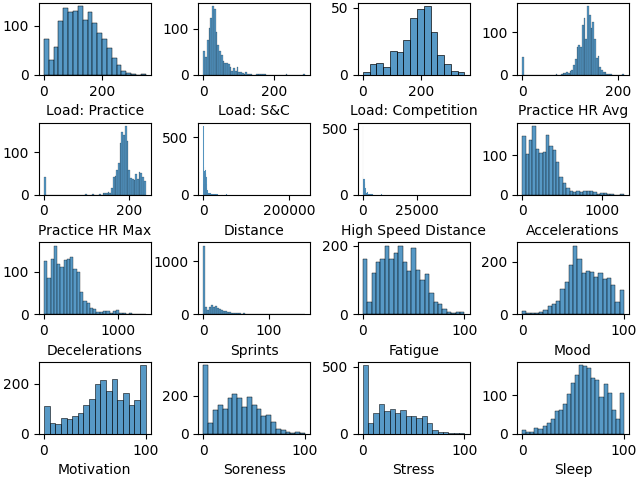
\includegraphics{../images/eda/eda_hist_all}
				\end{center}
				\caption{Histograms of all numeric variables in the provided data.}
				\label{fig:eda_hist_all}
			\end{figure}

			% A grid search was fit to each model, such that several different
			% estimators were employed and the best one selected for modeling
			% each outcome on the basis of five-fold cross-validation.

			Since the outcome variables in question appeared to be roughly
			gamma-distributed, we selected a gamma generalized linear model
			for the task of model-fitting.

			In the first part of the present analysis (see
			"Predicting Wellness Values using Workload and Sleep", below),
			fatigue, motivation, mood, and stress are treated as outcome
			variables; workload and sleep variables
			were treated as predictors. As outcomes, we
			assessed both the wellness variable and the change in that wellness
			variable to determine if there were effects on one or the other.

			In the second part of the analysis ("Predicting Sleep Disturbance using
			Workload Data", below), sleep moved out of its predictor status and
			was treated as an outcome to assess how
			training might affect sleep quality. Here, practice, strength and
			conditioning, and competition load were used as predictors.

			In the final part of the analysis ("Predicting Soreness using Workload,
			GPS, and Sleep", below), soreness was modeled using a larger
			subset of the data, involving practice, strength and conditioning, and
			competition load, distance, high speed distance, sprints, and sleep
			as predictors.

	\section{Results}
		
		\subsection{Exploratory Data Analysis}

			Investigations into the dataset indicated that the position groups
			are meaningfully different in terms of their duties and workload.
			For example, figure \ref{fig:eda_box_all_pos_group} indicates
			clear differences in variables such as motivation and decelerations.
			The number of pairwise comparisons that would be performed
			to test whether each group was meaningfully different from the others
			would likely have created a fairly drastic Bonferroni correction
			and was thus not included here.

			\begin{figure}
				\begin{center}
					% Thanks:
					% https://tex.stackexchange.com/questions/234441/latex-includegraphics-width-and-height
					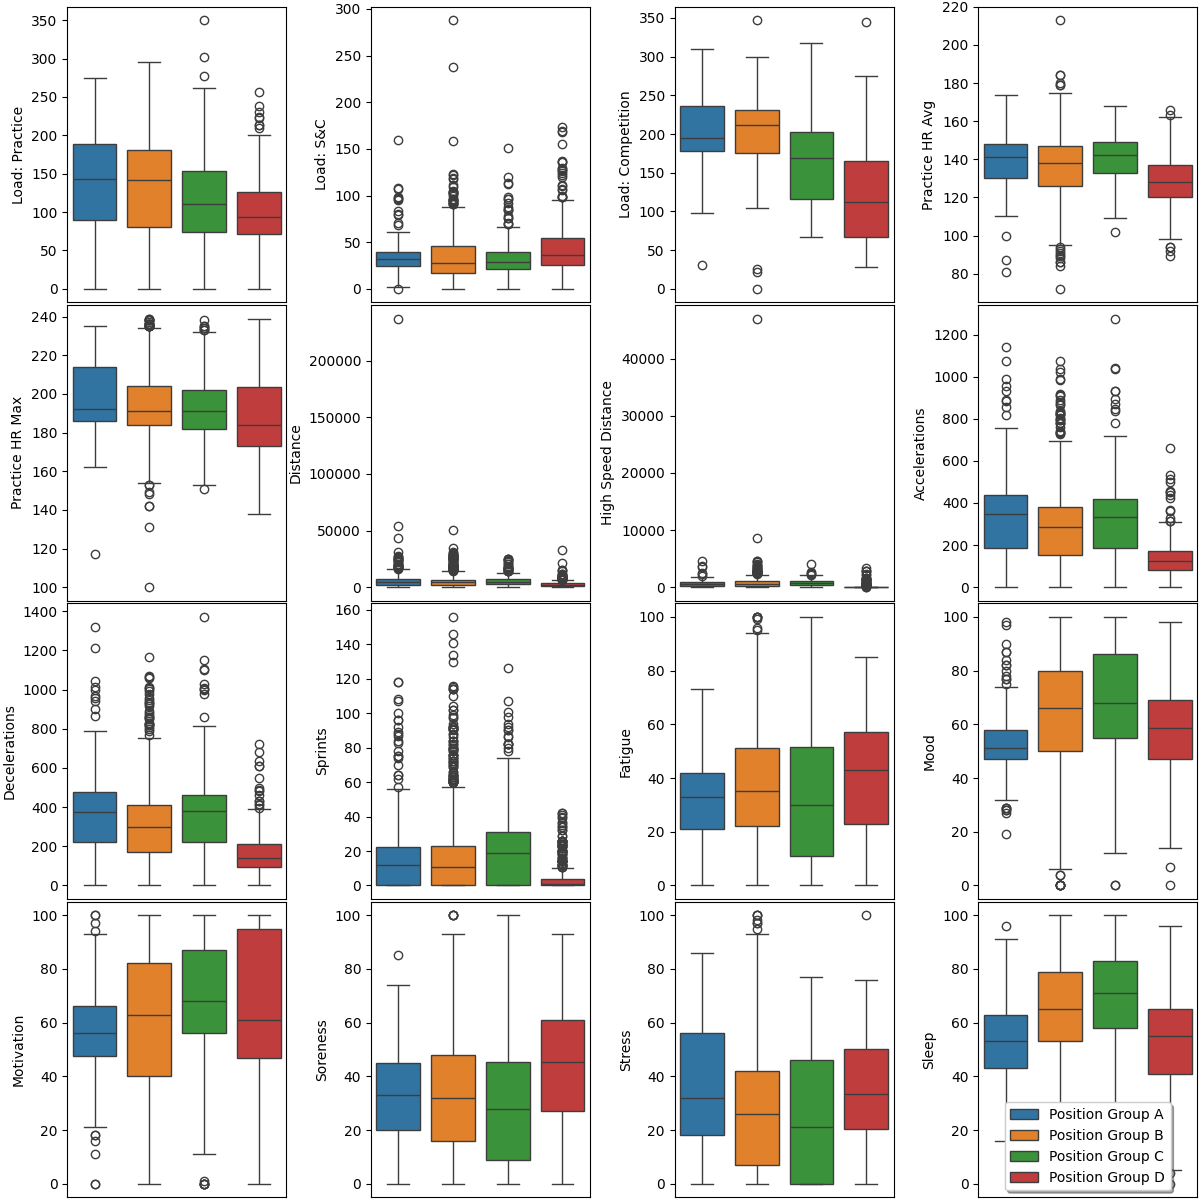
\includegraphics[
						width=16cm,
					]{../images/eda/eda_box_all_pos_group}
				\end{center}
				\label{fig:eda_box_all_pos_group}
				\caption{Box and whisker plots of each variable for the four
				position groups. Each plot displays distributions for position
				groups A, B, C, and D respectively, from left to right.}
			\end{figure}

			Several variables were found to be highly correlated with one
			another such that they could not both be included in a model
			together as predictors without undermining the ability to make
			inferences about the effect of any one of those variables on
			the outcome. These were as follows:

			\begin{itemize}
				\item Practice load and average practice heart rate.
				\item Distance and accelerations.
				\item Distance and decelerations.
				\item Accelerations and decelerations.
			\end{itemize}

			From this information, it was inferred that practice load
			and average heart rate probably capture much of the same
			information, which makes sense physiologically. Furthermore,
			simply because of the nature of GPS data, the correlations
			between distance and the velocity change values made sense.
			As a result, include practice load and heart rate were not
			included in
			the same set of predictors during modeling, nor were 
			any two of distance, accelerations, and decelerations. Because
			of its overall intuitive quality and descriptiveness,
			distance was selected among those three as the predictor that
			would be included when relevant.

			Exploratory data analysis also revealed that none of the wellness
			variables appeared to be normally distributed \ref{fig:eda_hist_all}.
			Since the fatigue, soreness, and stress variables appeared to roughly follow
			a gamma distribution (or reversed gamma distribution),
			a gamma generalized linear model with the log
			link function was included among the models that were fit in the grid
			search for each outcome variable. The log link function was chosen
			due to matrix multiplication issues that occurred in \texttt{NumPy}'s
			and R's \texttt{glm} package code, which were not able to fit the data
			with some of the options they provided. This is likely due to some
			large values in the dataset that created consequently large matrix products.
			Using the log linking function circumvented this problem.

			%These models, however, failed to converge first due a matrix multiplication
			%error in \texttt{NumPy}. We then moved on and tried to implement them in
			%R, thinking that there may have been some issue with \texttt{Numpy}'s backend
			%implementation. This also resulted in poor model convergence. As a
			%consequence, we pivoted to other models. These included Bayesian Ridge
			%regression and support vector machines.

		\subsection{Predicting Wellness Values using Workload and Sleep}

			% Workload, sleep, and fatigue.
			\begin{figure}
				\begin{center}
					% Thanks:
					% https://tex.stackexchange.com/questions/234441/latex-includegraphics-width-and-height
					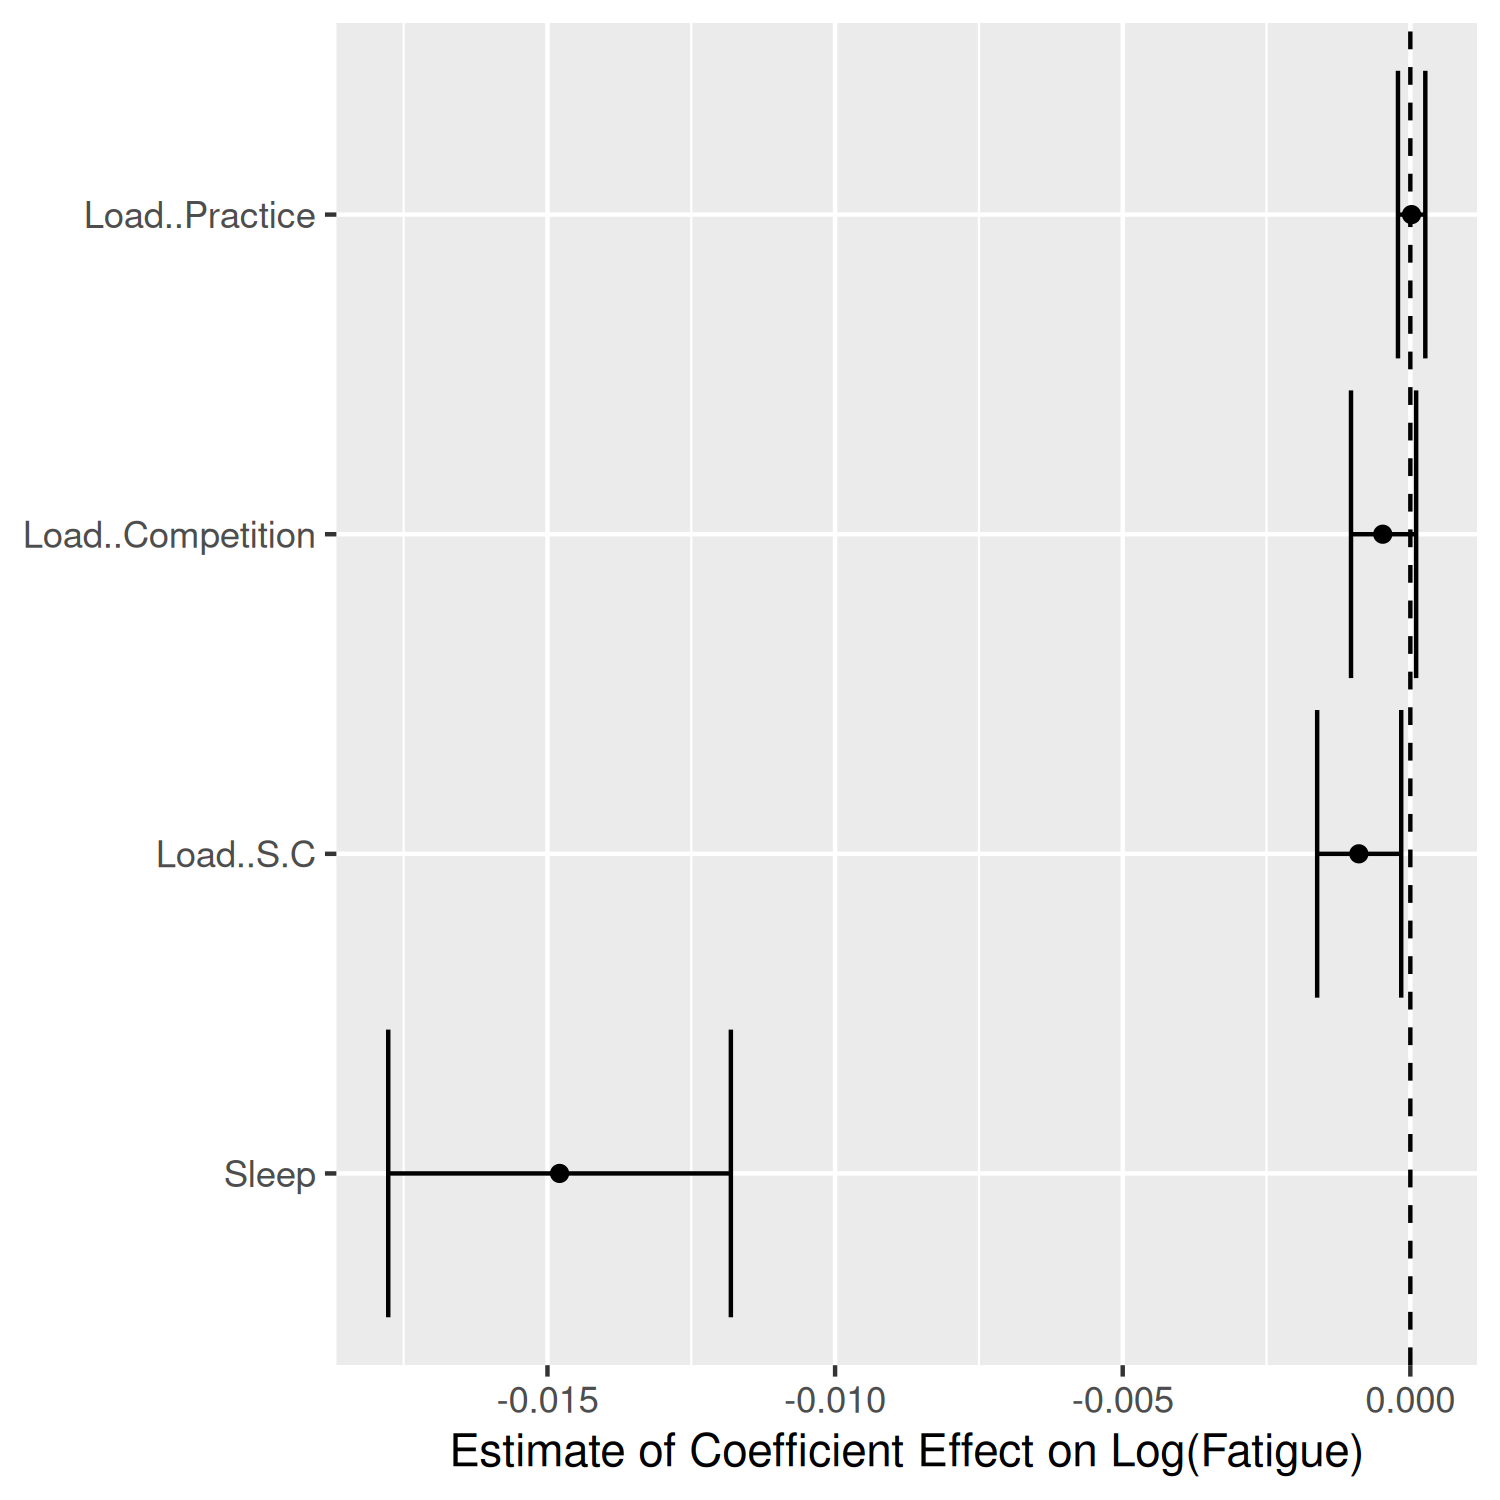
\includegraphics[
						width=12cm,
					]{../out/analysis_weekly_workload/workload_sleep_fatigue/coef.png}
				\end{center}
				\caption{Coefficient magnitudes for gamma generalized linear regression
				of fatigue based on sleep and workload data.}
				\label{fig:weekly_workload_sleep_fatigue_coef}
			\end{figure}

			\begin{figure}
				\begin{center}
					% Thanks:
					% https://tex.stackexchange.com/questions/234441/latex-includegraphics-width-and-height
					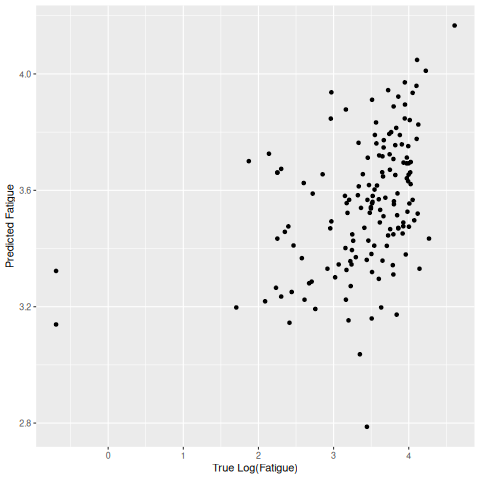
\includegraphics[
						width=12cm,
					]{../out/analysis_weekly_workload/workload_sleep_fatigue/scatter_pred_true.png}
				\end{center}
				\caption{
					Scatterplot of predicted and true log-transformed outcome
					values for gamma generalized linear regression
					of fatigue based on sleep and workload data.
				}
				\label{fig:weekly_workload_sleep_fatigue_scatter}
			\end{figure}

			% Workload, sleep, and fatigue delta.
			\begin{figure}
				\begin{center}
					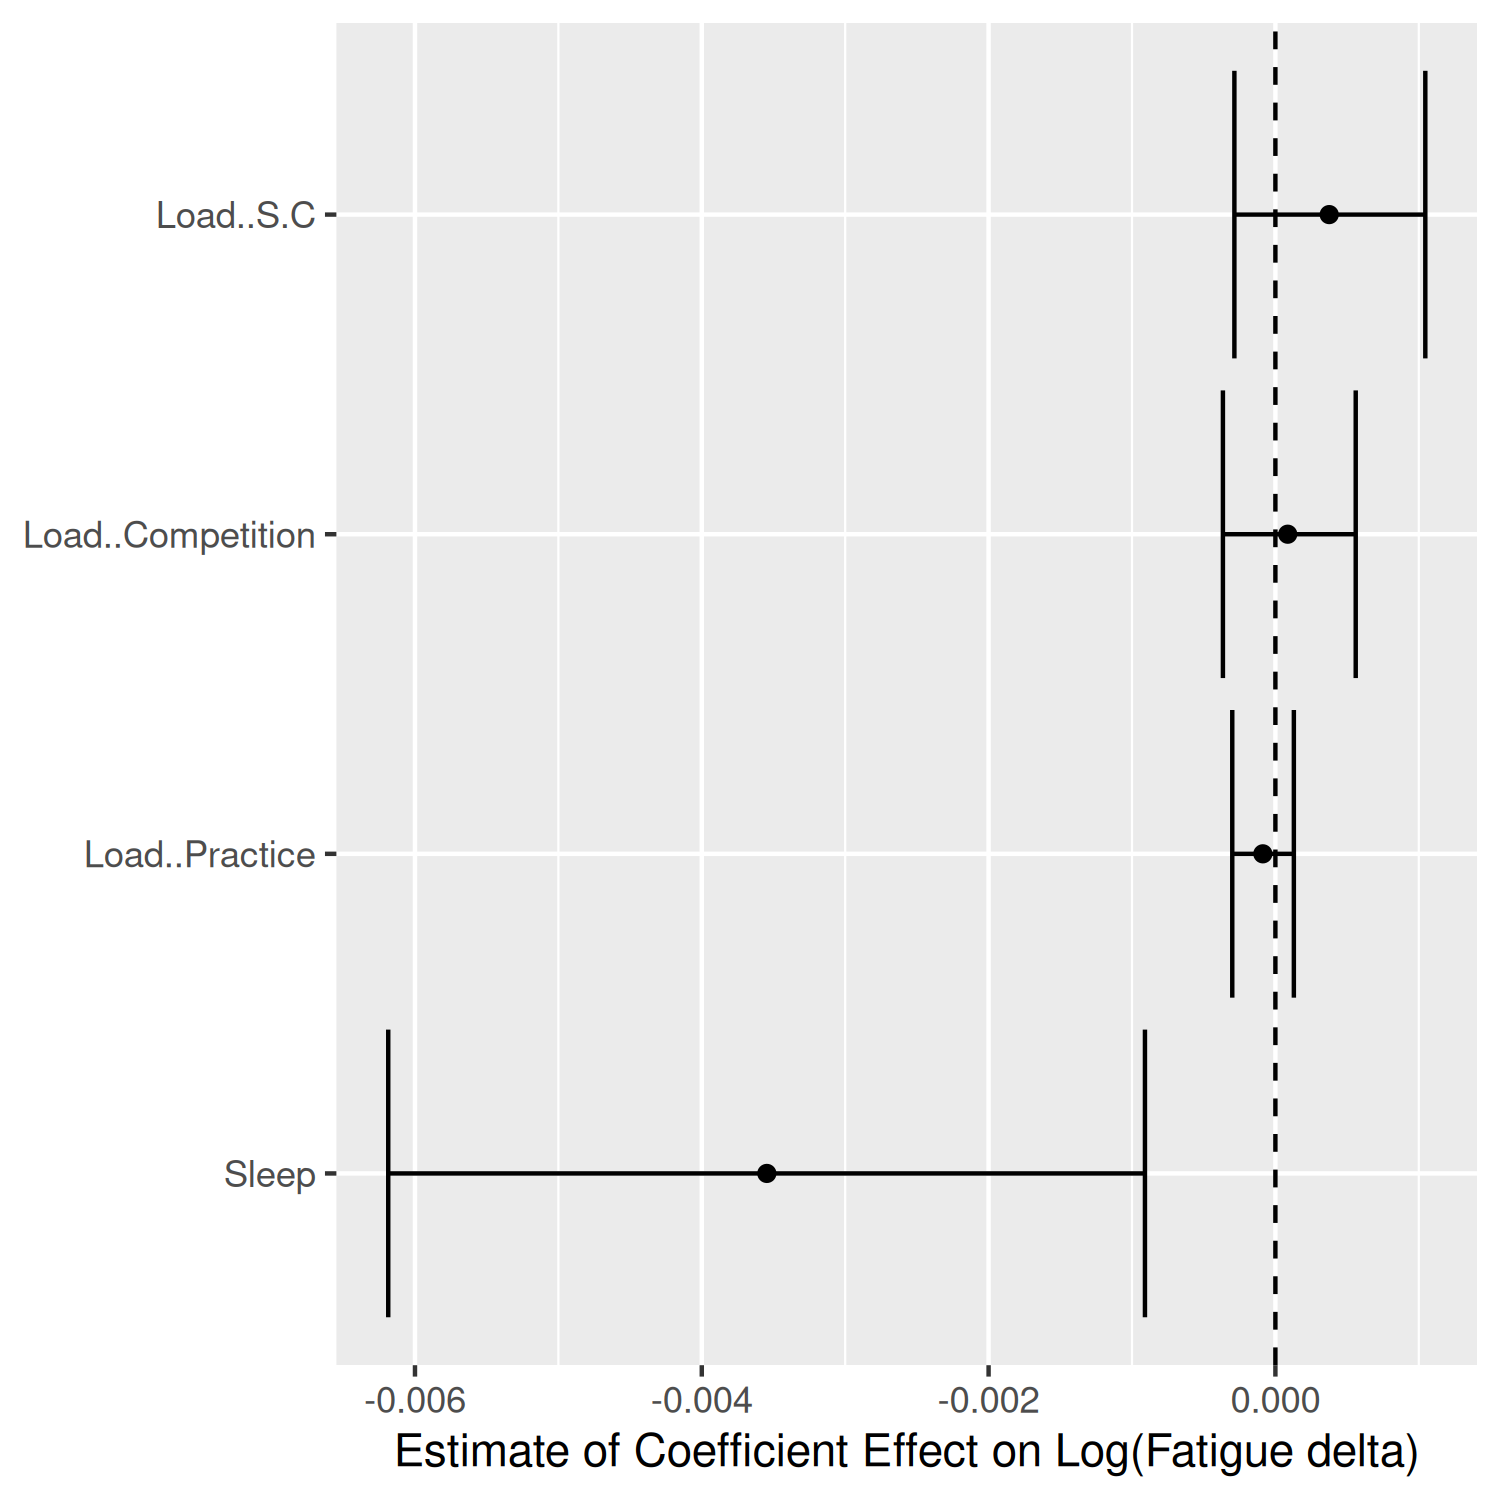
\includegraphics[
						width=12cm,
					]{../out/analysis_weekly_workload/workload_sleep_fatigue_delta/coef.png}
				\end{center}
				\caption{Coefficient magnitudes for gamma generalized linear regression
				of fatigue delta based on sleep and workload data.}
				\label{fig:weekly_workload_sleep_fatigue_delta_coef}
			\end{figure}

			\begin{figure}
				\begin{center}
					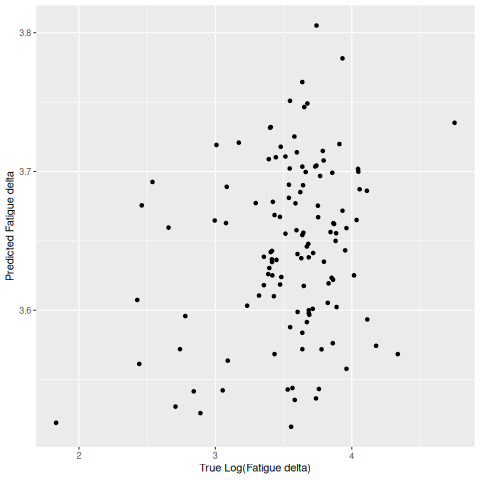
\includegraphics[
						width=12cm,
					]{../out/analysis_weekly_workload/workload_sleep_fatigue_delta/scatter_pred_true.png}
				\end{center}
				\caption{
					Scatterplot of predicted and true log-transformed outcome
					values for gamma generalized linear regression
					of fatigue delta based on sleep and workload data.
				}
				\label{fig:weekly_workload_sleep_fatigue_delta_scatter}
			\end{figure}

			% Workload, sleep, and mood.
			\begin{figure}
				\begin{center}
					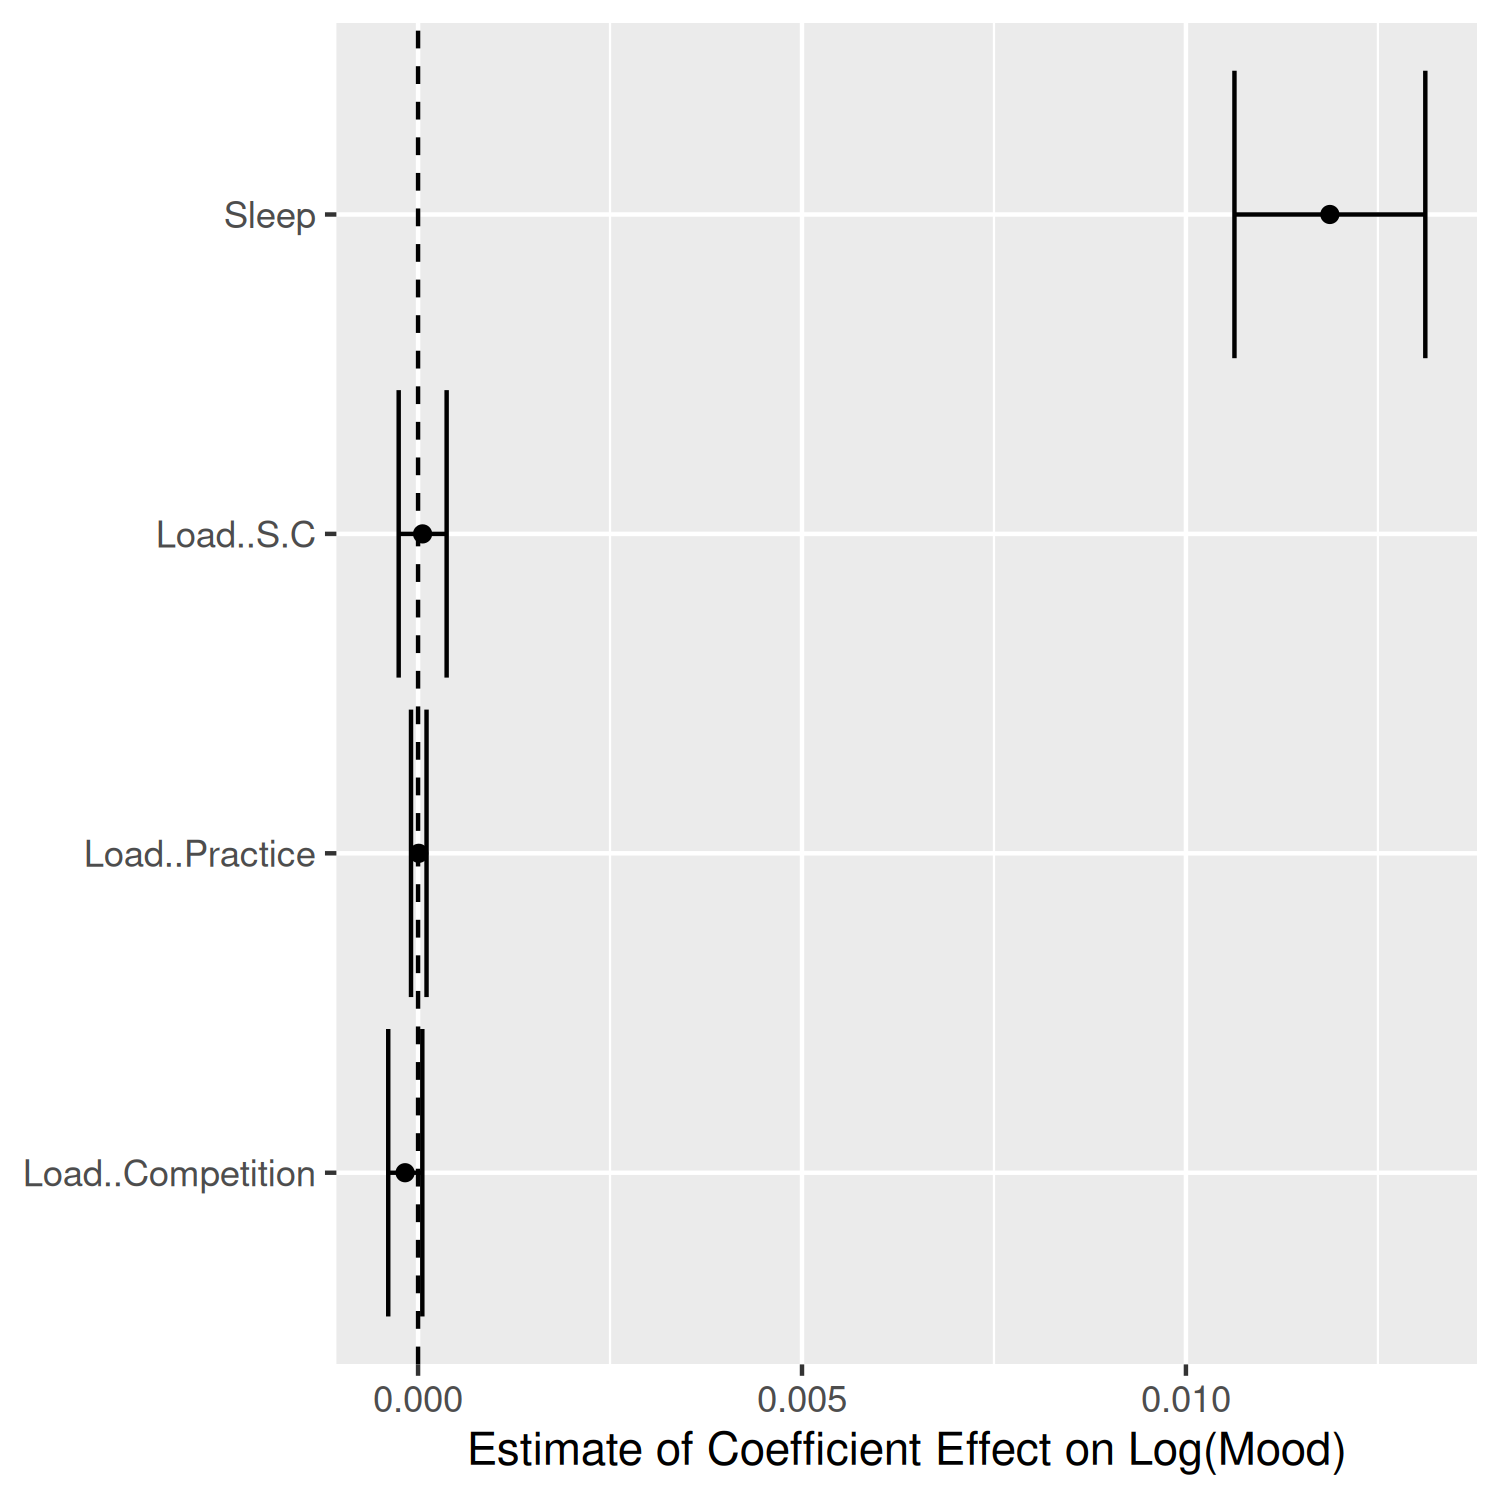
\includegraphics[
						width=12cm,
					]{../out/analysis_weekly_workload/workload_sleep_mood/coef.png}
				\end{center}
				\caption{Coefficient magnitudes for gamma generalized linear regression
				of mood based on sleep and workload data.}
				\label{fig:weekly_workload_sleep_mood_coef}
			\end{figure}

			\begin{figure}
				\begin{center}
					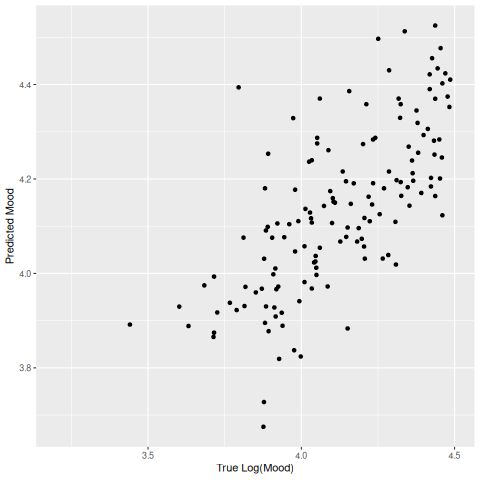
\includegraphics[
						width=12cm,
					]{../out/analysis_weekly_workload/workload_sleep_mood/scatter_pred_true.png}
				\end{center}
				\caption{
					Scatterplot of predicted and true log-transformed outcome
					values for gamma generalized linear regression
					of mood based on sleep and workload data.
				}
				\label{fig:weekly_workload_sleep_mood_scatter}
			\end{figure}

			% Workload, sleep, and mood delta.

			\begin{figure}
				\begin{center}
					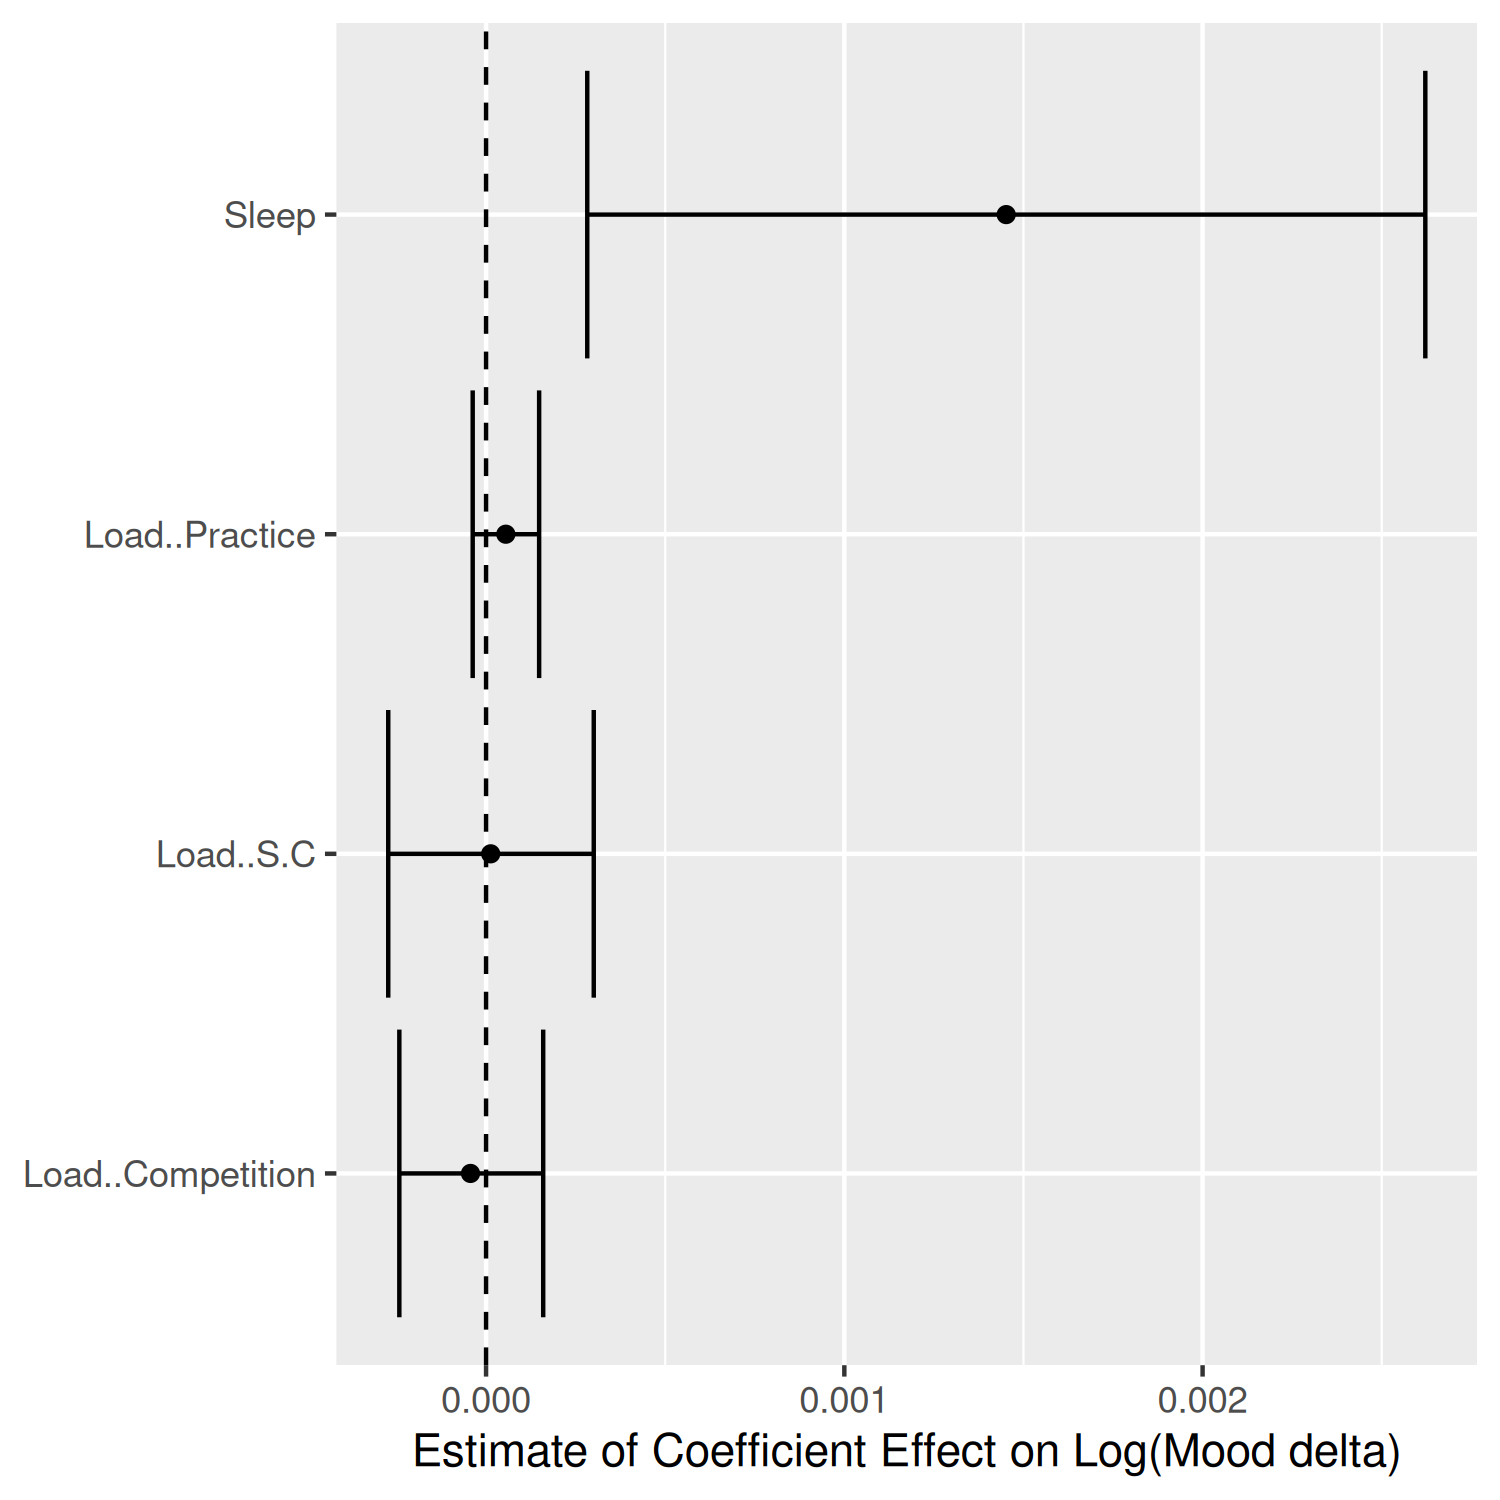
\includegraphics[
						width=12cm,
					]{../out/analysis_weekly_workload/workload_sleep_mood_delta/coef.png}
				\end{center}
				\caption{Coefficient magnitudes for gamma generalized linear regression
				of mood delta based on sleep and workload data.}
				\label{fig:weekly_workload_sleep_mood_delta_coef}
			\end{figure}

			\begin{figure}
				\begin{center}
					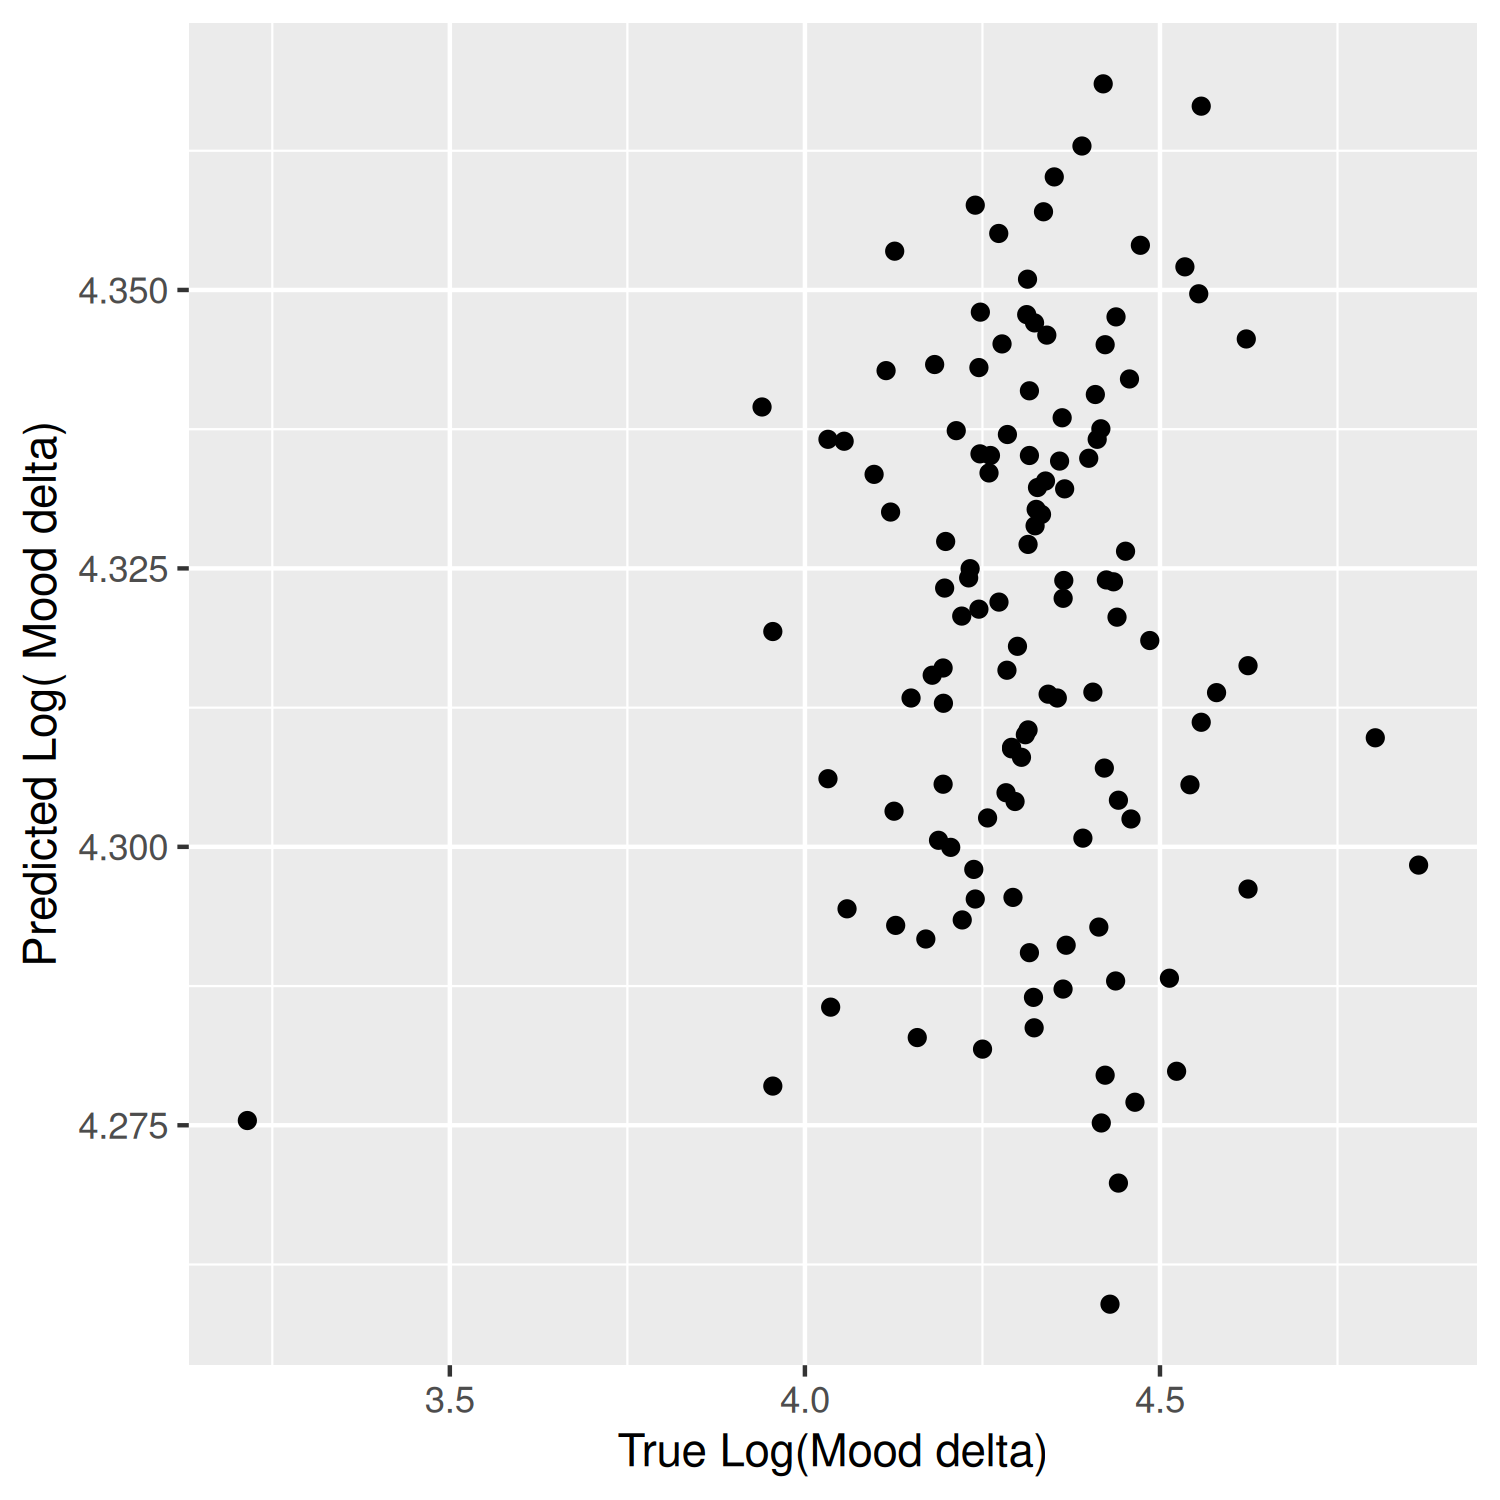
\includegraphics[
						width=12cm,
					]{../out/analysis_weekly_workload/workload_sleep_mood_delta/scatter_pred_true.png}
				\end{center}
				\caption{
					Scatterplot of predicted and true log-transformed outcome
					values for gamma generalized linear regression
					of mood delta based on sleep and workload data.
				}
				\label{fig:weekly_workload_sleep_mood_delta_scatter}
			\end{figure}

			% Workload, sleep, and motivation.

			\begin{figure}
				\begin{center}
					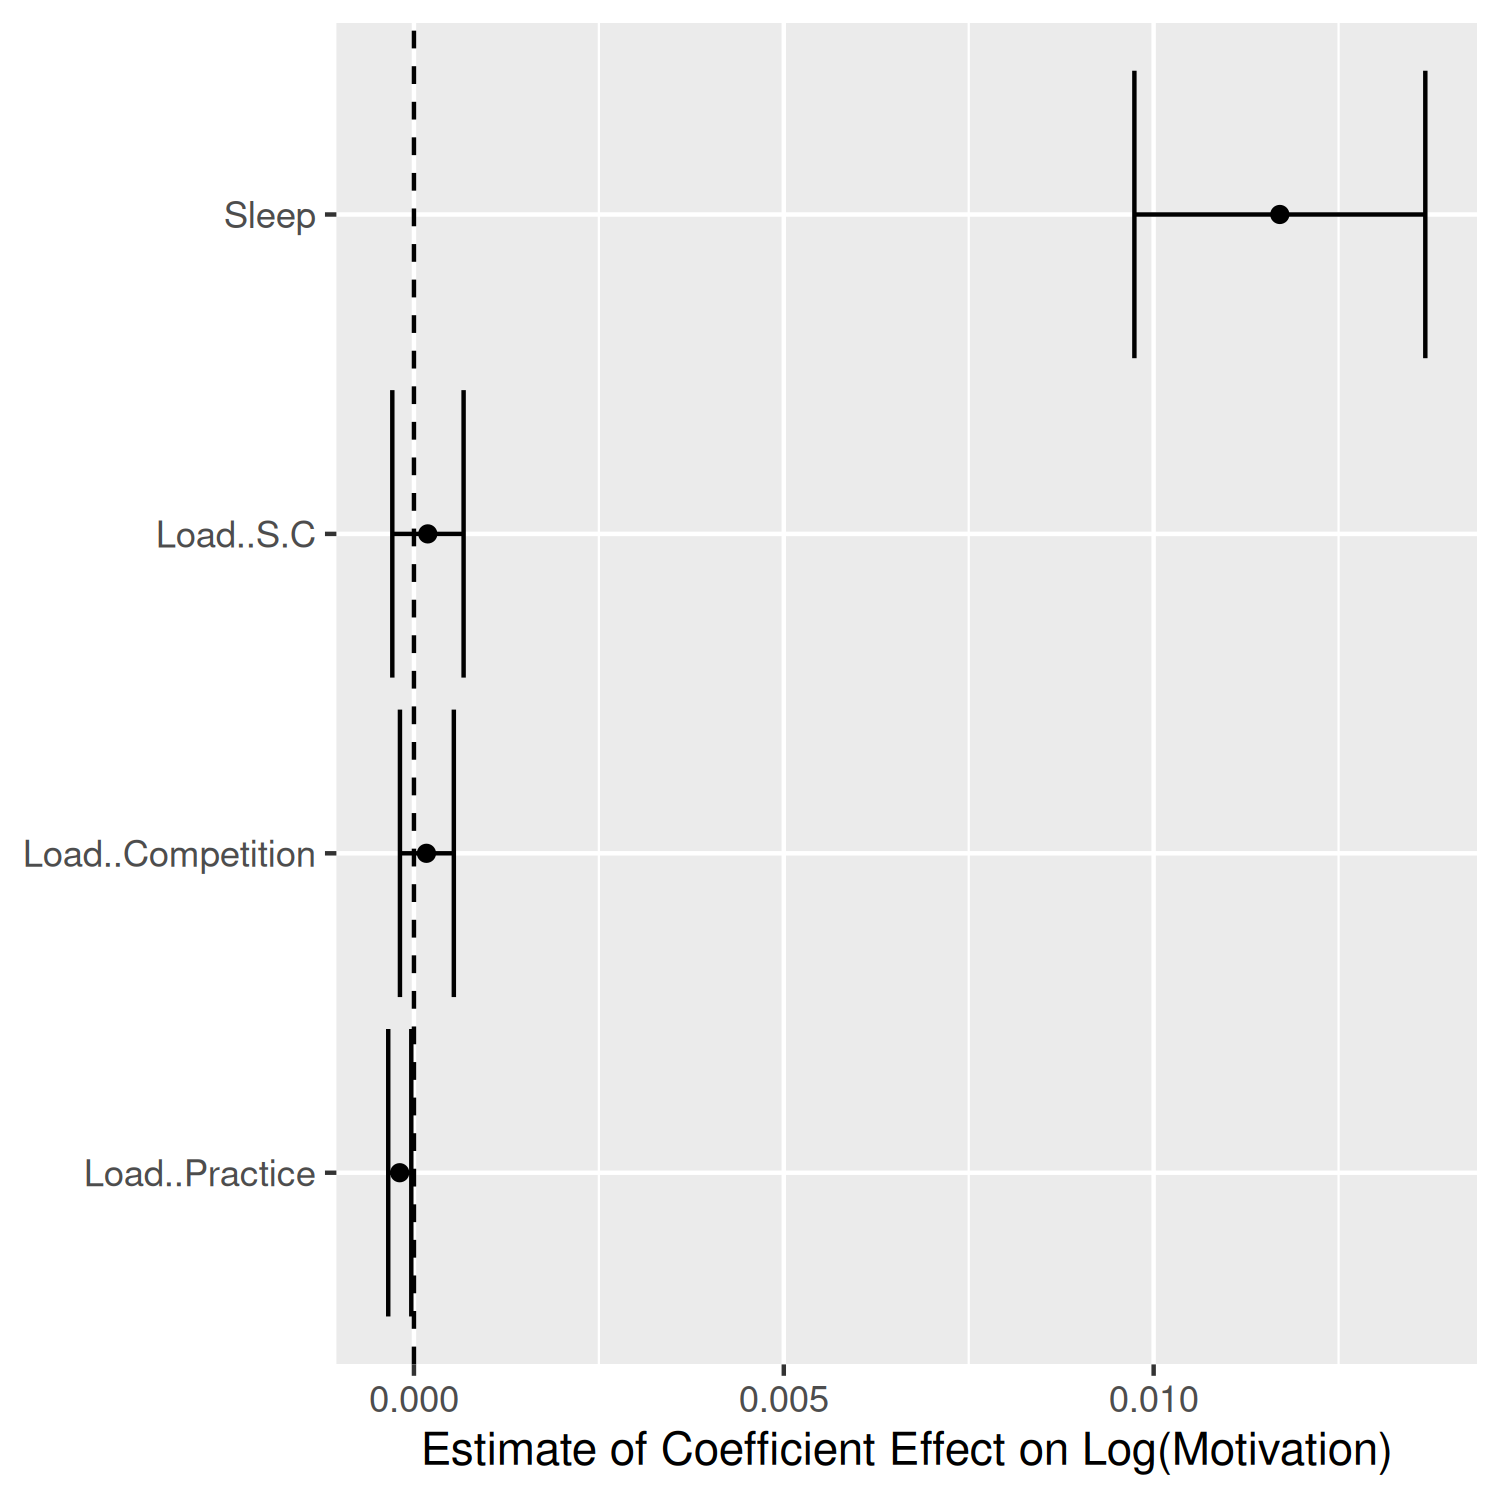
\includegraphics[
						width=12cm,
					]{../out/analysis_weekly_workload/workload_sleep_motivation/coef.png}
				\end{center}
				\caption{Coefficient magnitudes for gamma generalized linear regression
				of motivation based on sleep and workload data.}
				\label{fig:weekly_workload_sleep_motivation_coef}
			\end{figure}

			\begin{figure}
				\begin{center}
					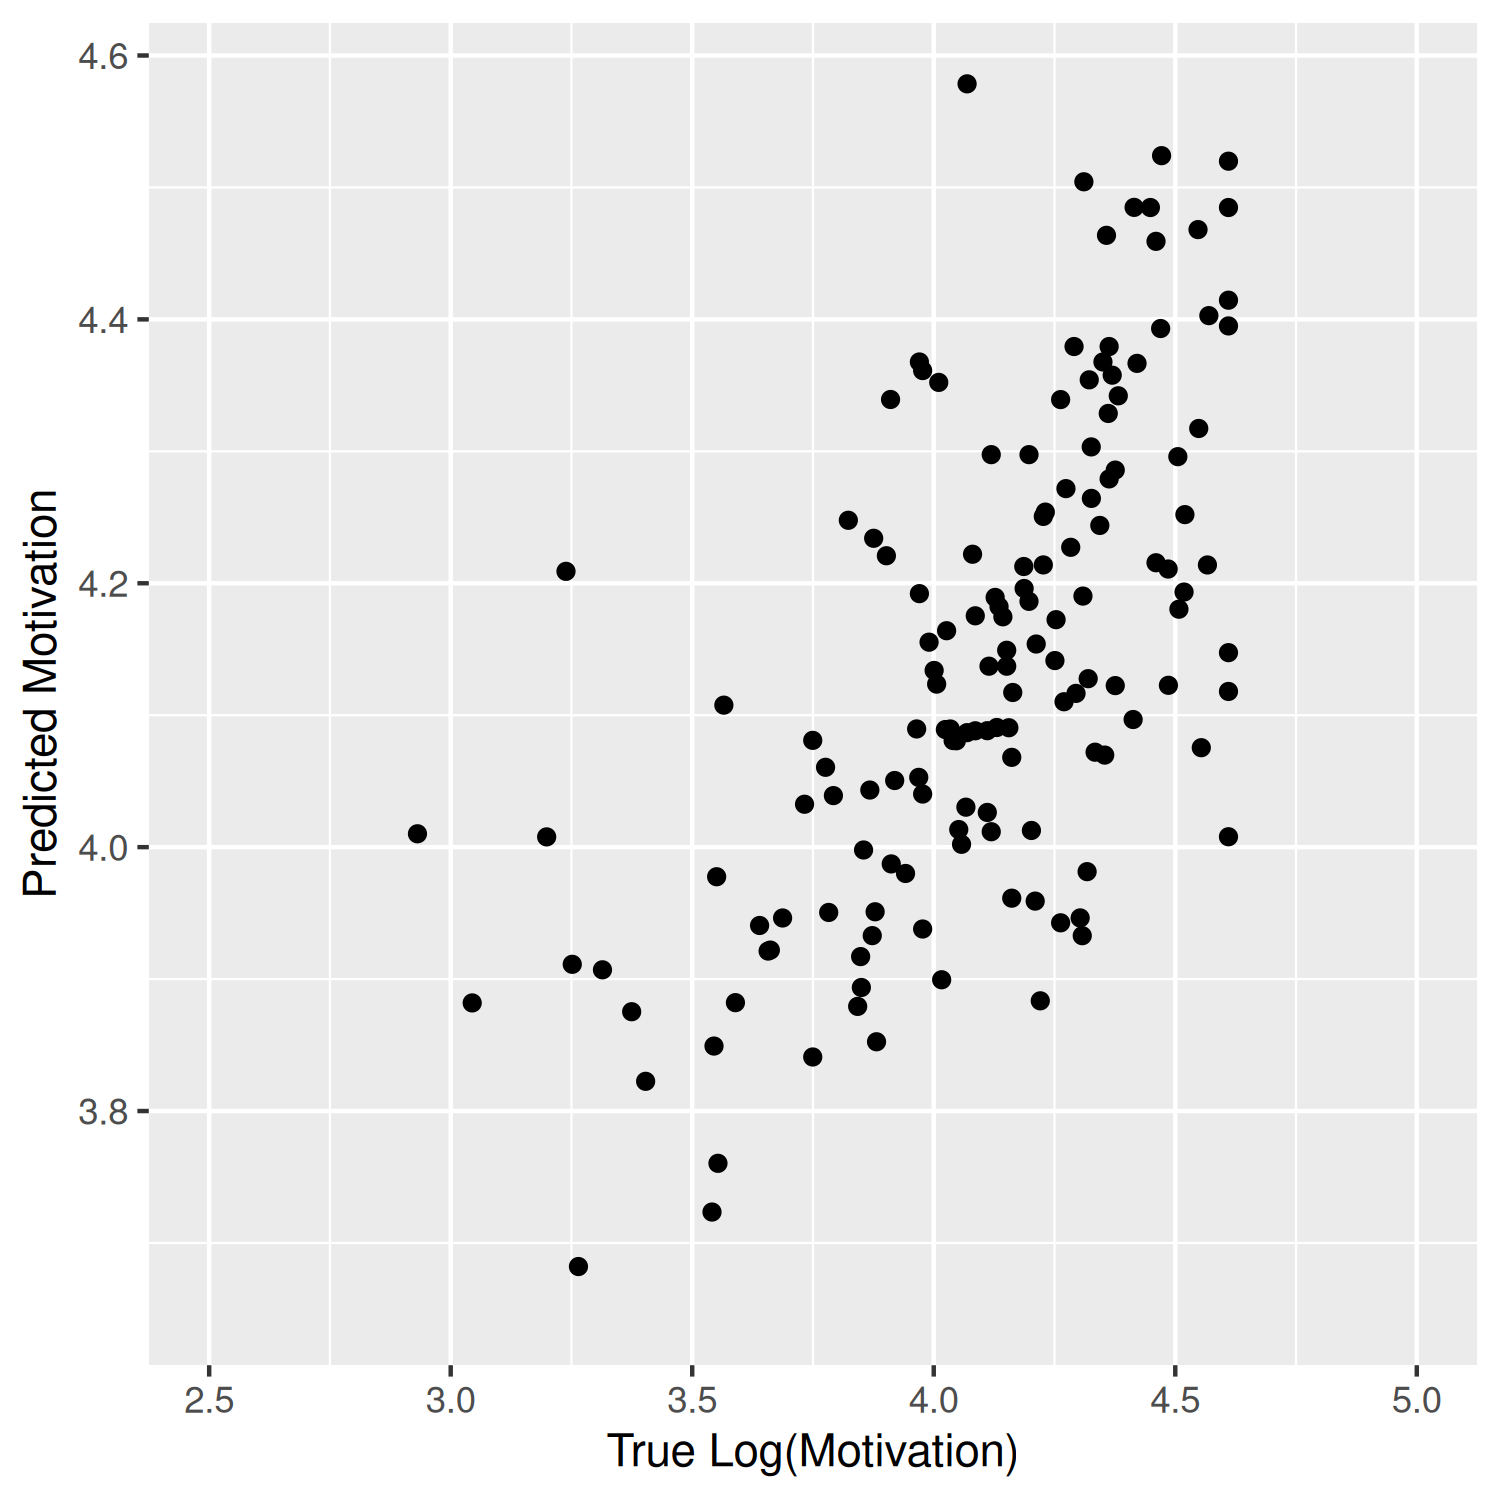
\includegraphics[
						width=12cm,
					]{../out/analysis_weekly_workload/workload_sleep_motivation/scatter_pred_true.png}
				\end{center}
				\caption{
					Scatterplot of predicted and true log-transformed outcome
					values for gamma generalized linear regression
					of motivation based on sleep and workload data.
				}
				\label{fig:weekly_workload_sleep_motivation_scatter}
			\end{figure}

			% Workload, sleep, and motivation delta.

			\begin{figure}
				\begin{center}
					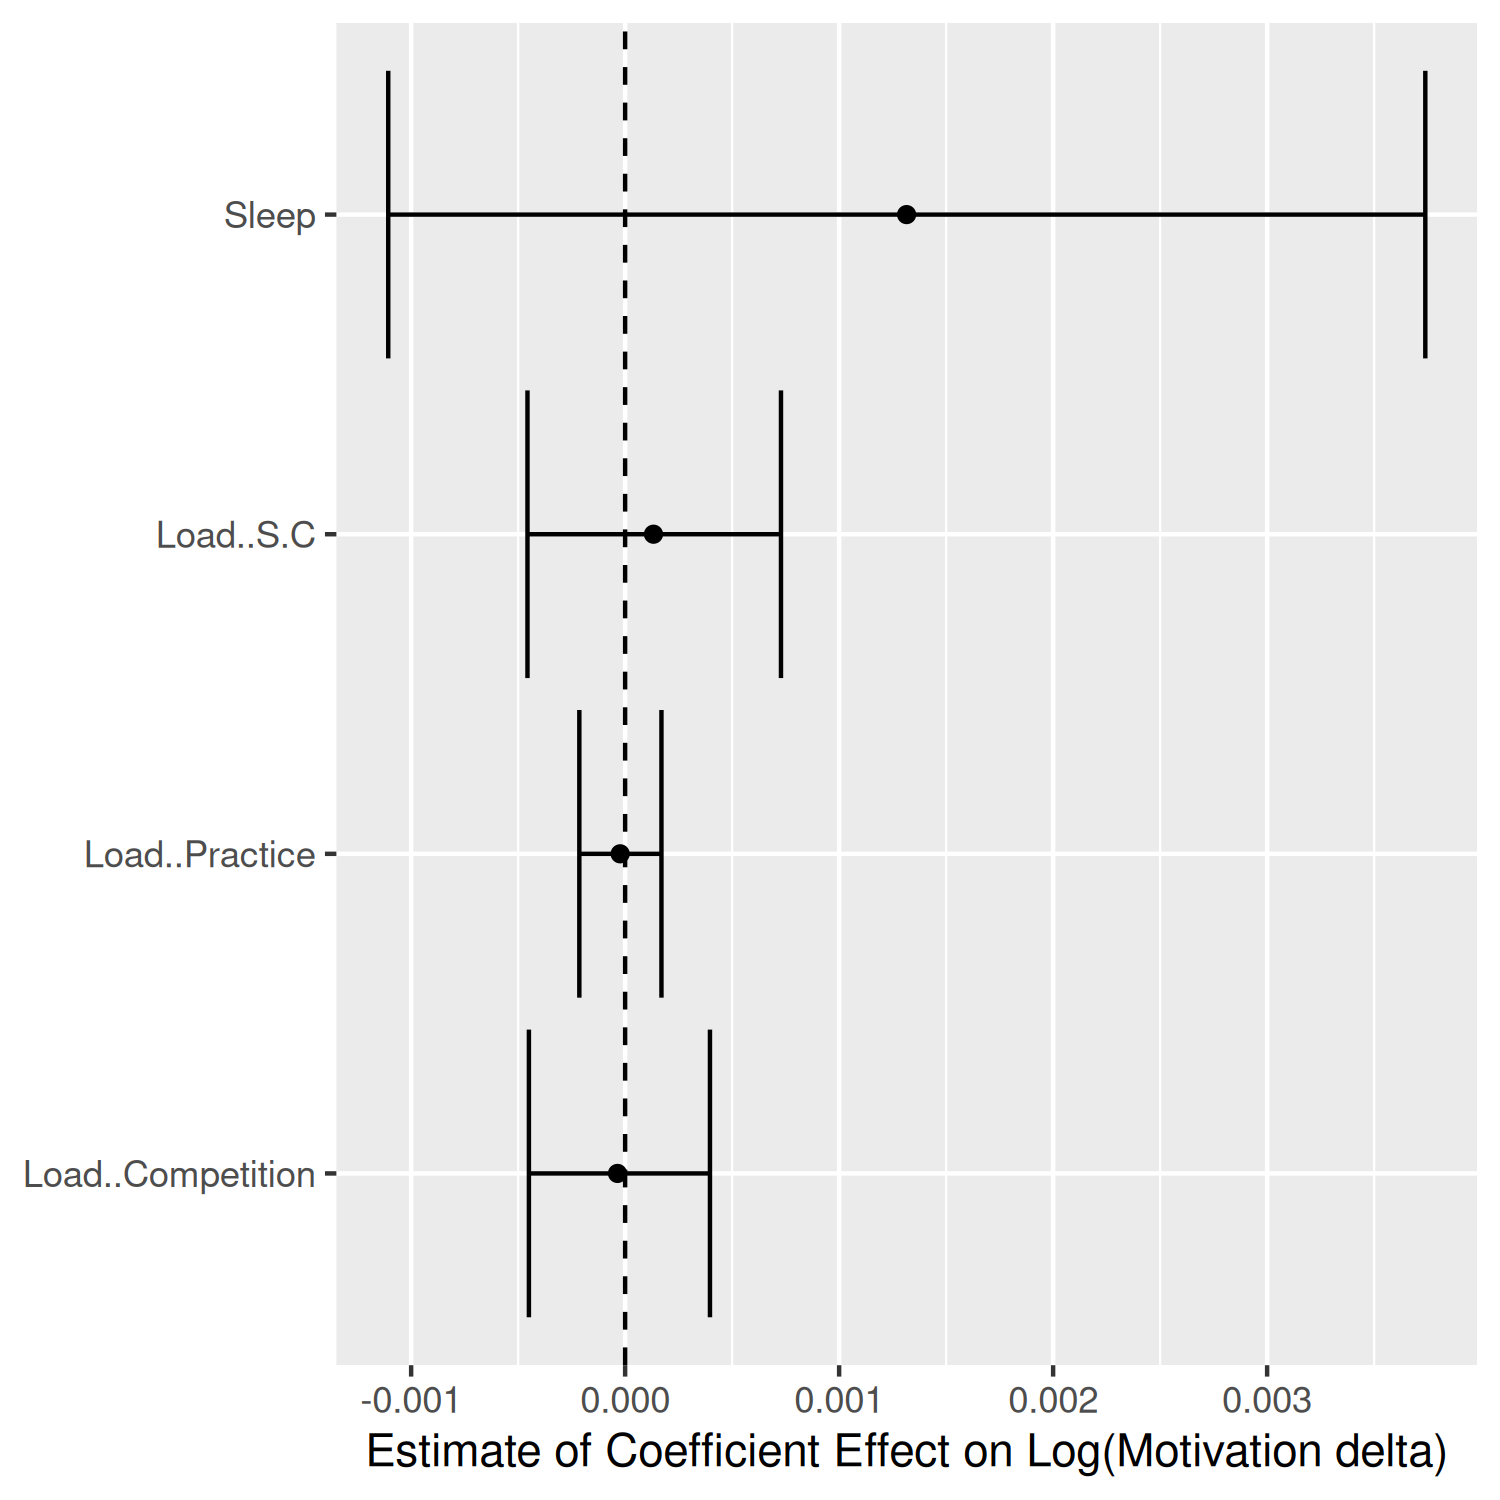
\includegraphics[
						width=12cm,
					]{../out/analysis_weekly_workload/workload_sleep_motivation_delta/coef.png}
				\end{center}
				\caption{Coefficient magnitudes for gamma generalized linear regression
				of motivation delta based on sleep and workload data.}
				\label{fig:weekly_workload_sleep_motivation_delta_coef}
			\end{figure}

			\begin{figure}
				\begin{center}
					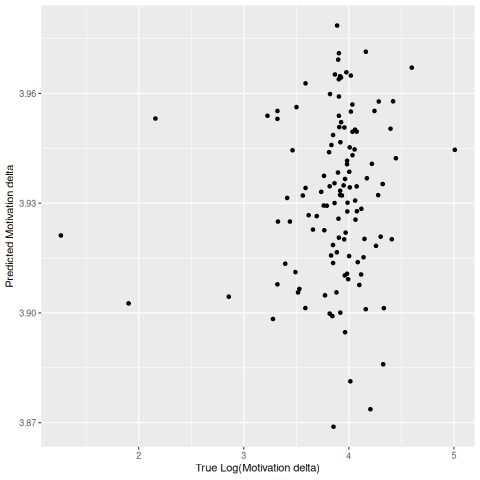
\includegraphics[
						width=12cm,
					]{../out/analysis_weekly_workload/workload_sleep_motivation_delta/scatter_pred_true.png}
				\end{center}
				\caption{
					Scatterplot of predicted and true log-transformed outcome
					values for gamma generalized linear regression
					of motivation delta based on sleep and workload data.
				}
				\label{fig:weekly_workload_sleep_motivation_delta_scatter}
			\end{figure}

			% Workload, sleep, and stress.

			\begin{figure}
				\begin{center}
					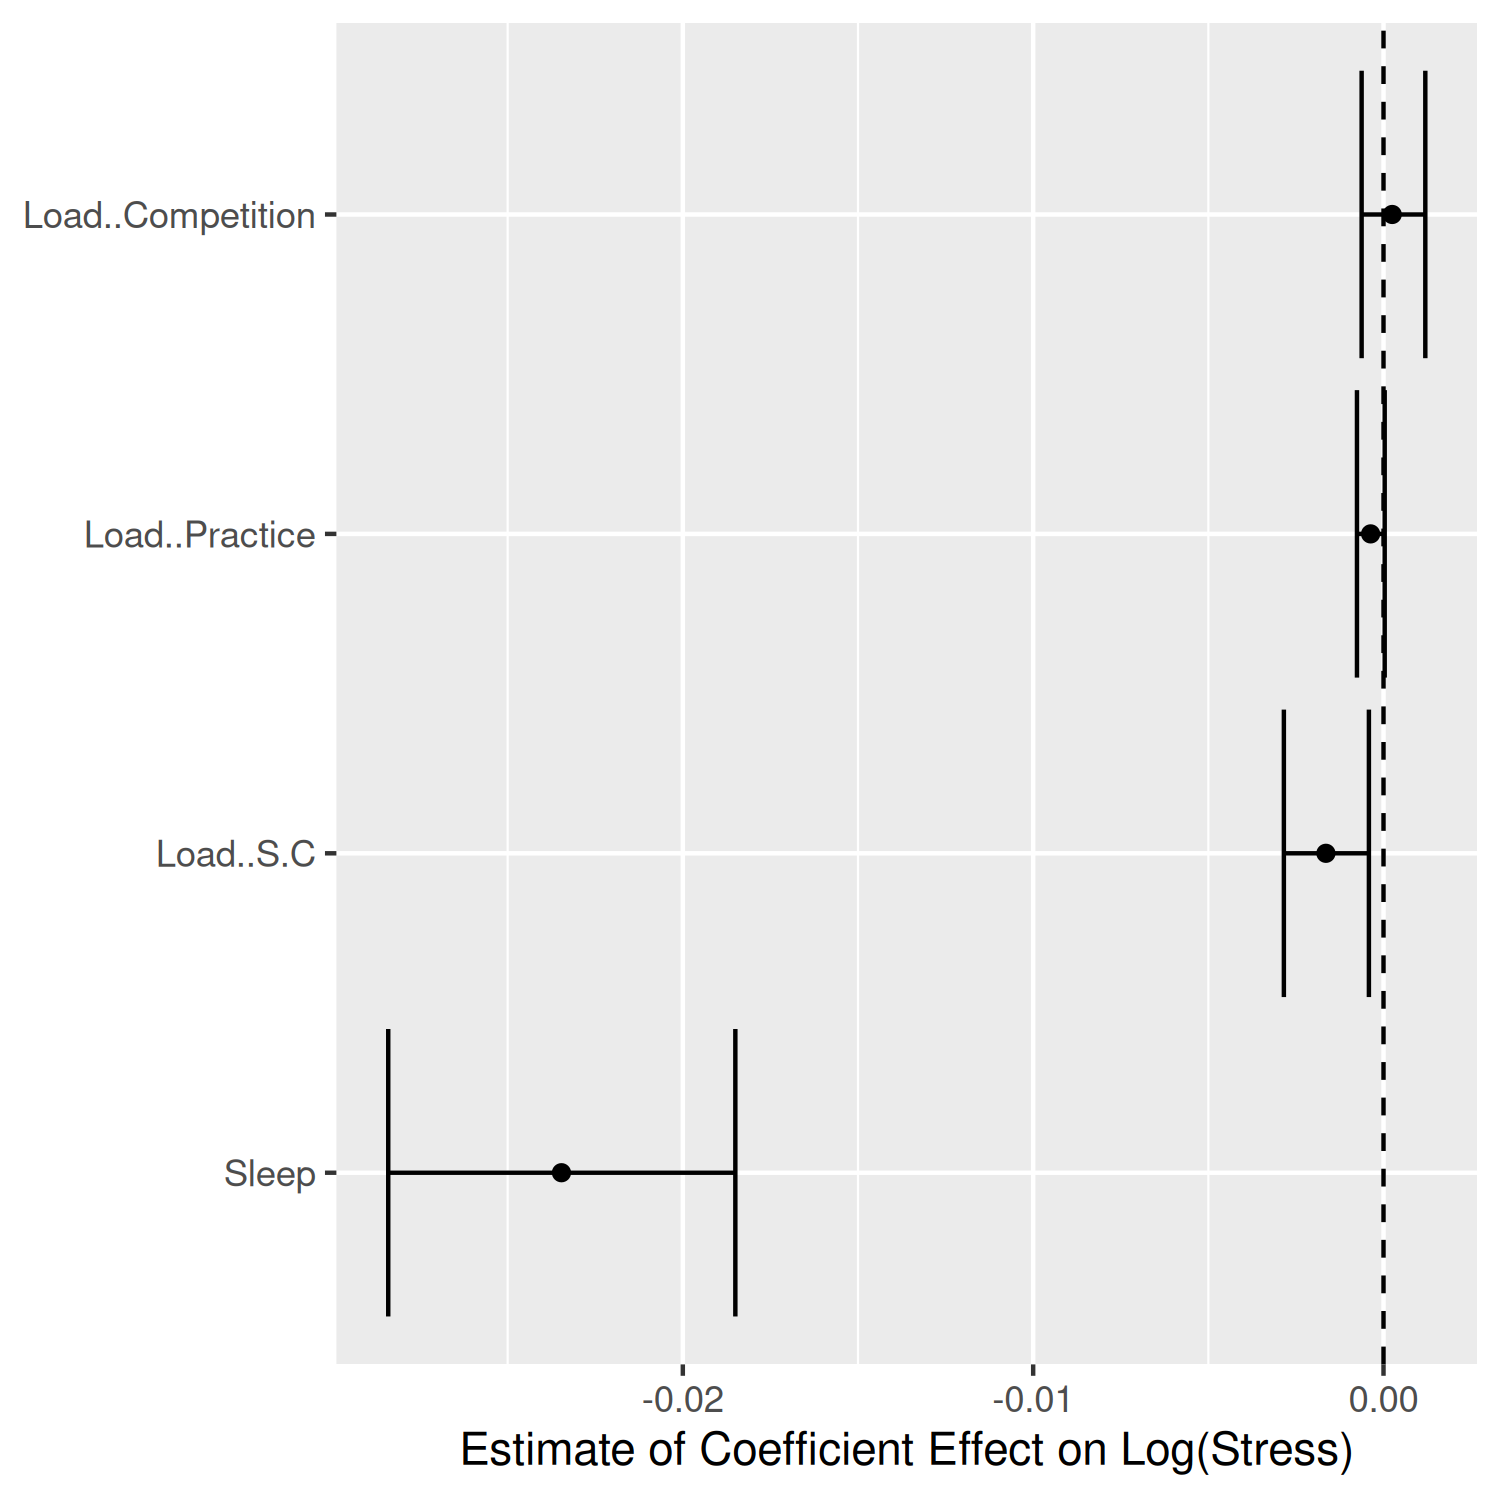
\includegraphics[
						width=12cm,
					]{../out/analysis_weekly_workload/workload_sleep_stress/coef.png}
				\end{center}
				\caption{Coefficient magnitudes for gamma generalized linear regression
				of stress based on sleep and workload data.}
				\label{fig:weekly_workload_sleep_stress_coef}
			\end{figure}

			\begin{figure}
				\begin{center}
					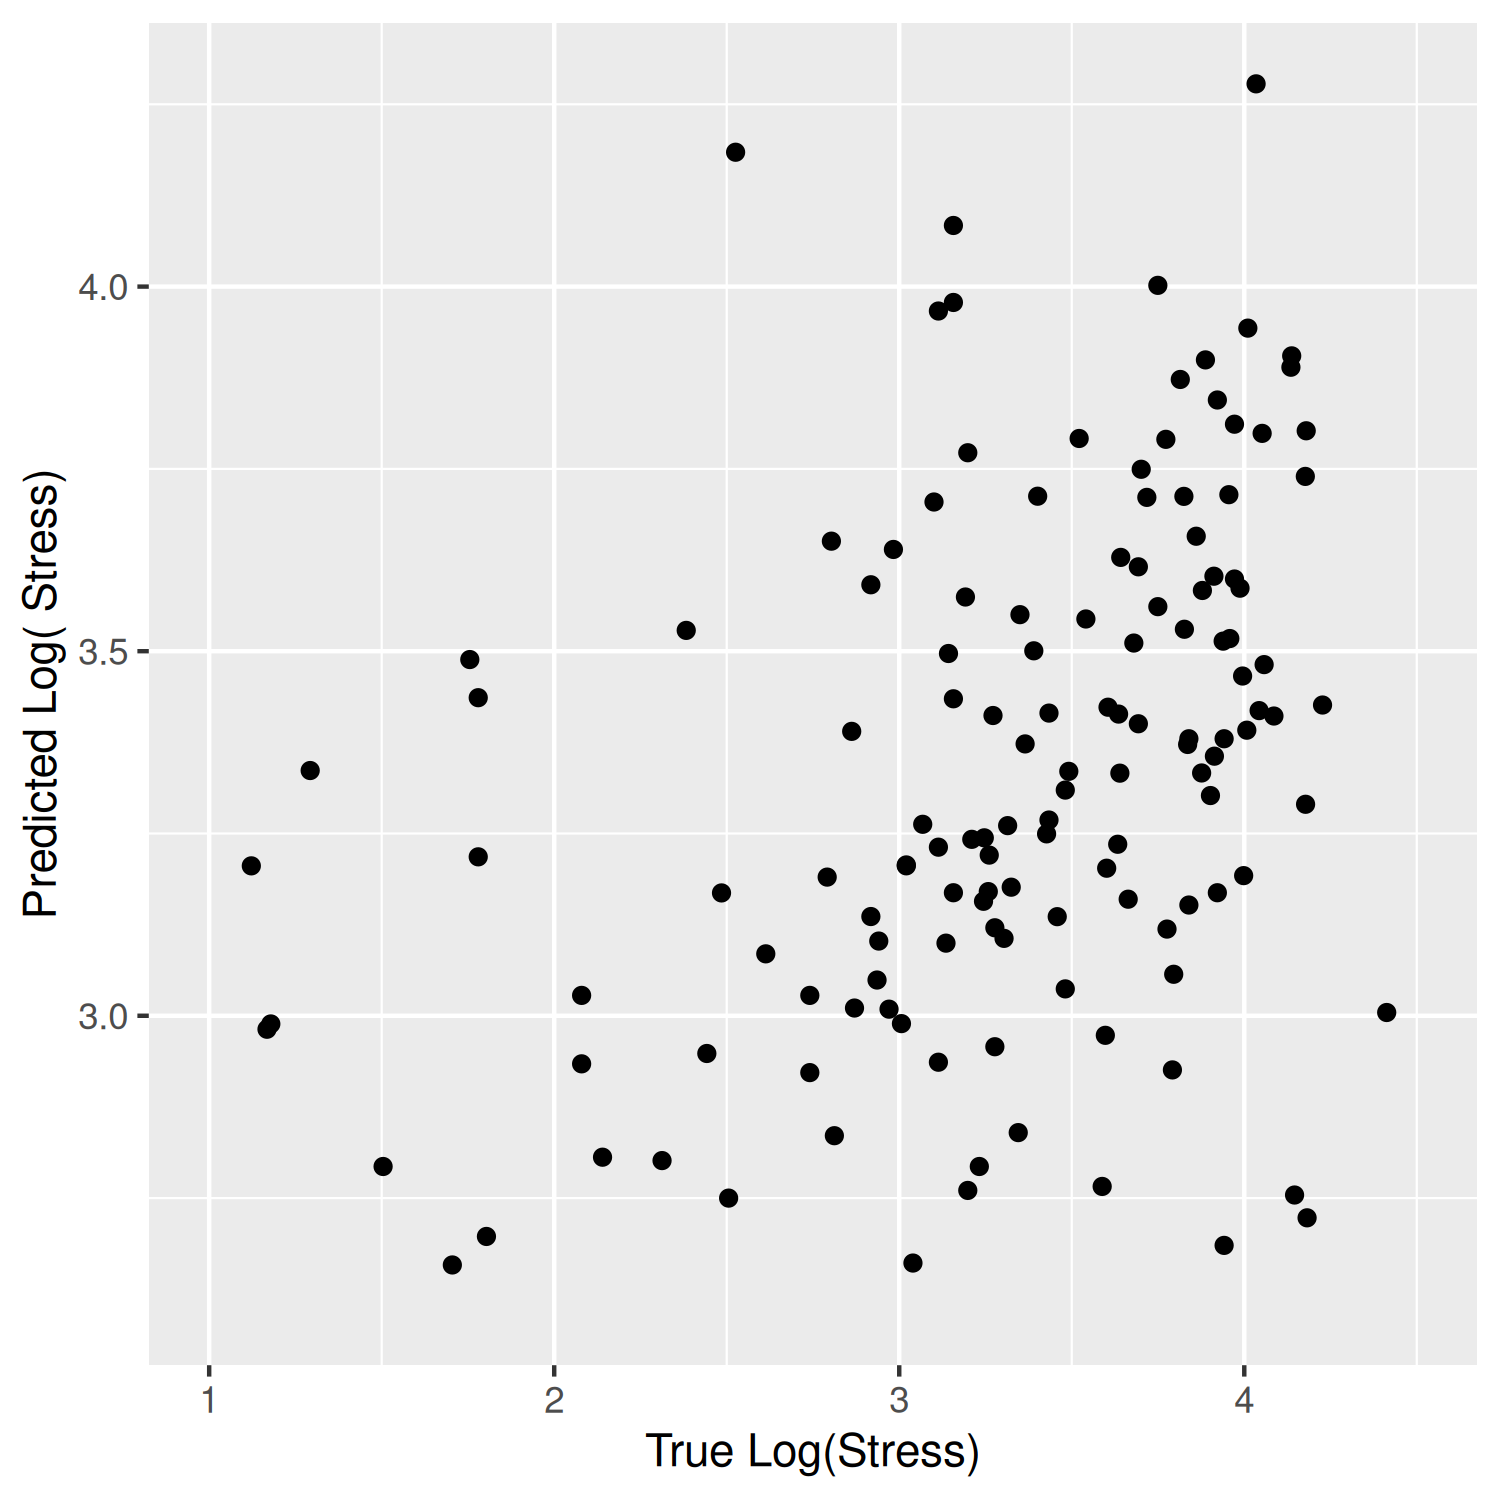
\includegraphics[
						width=12cm,
					]{../out/analysis_weekly_workload/workload_sleep_stress/scatter_pred_true.png}
				\end{center}
				\caption{
					Scatterplot of predicted and true log-transformed outcome
					values for gamma generalized linear regression
					of stress based on sleep and workload data.
				}
				\label{fig:weekly_workload_sleep_stress_scatter}
			\end{figure}

			% Workload, sleep, and stress delta.

			\begin{figure}
				\begin{center}
					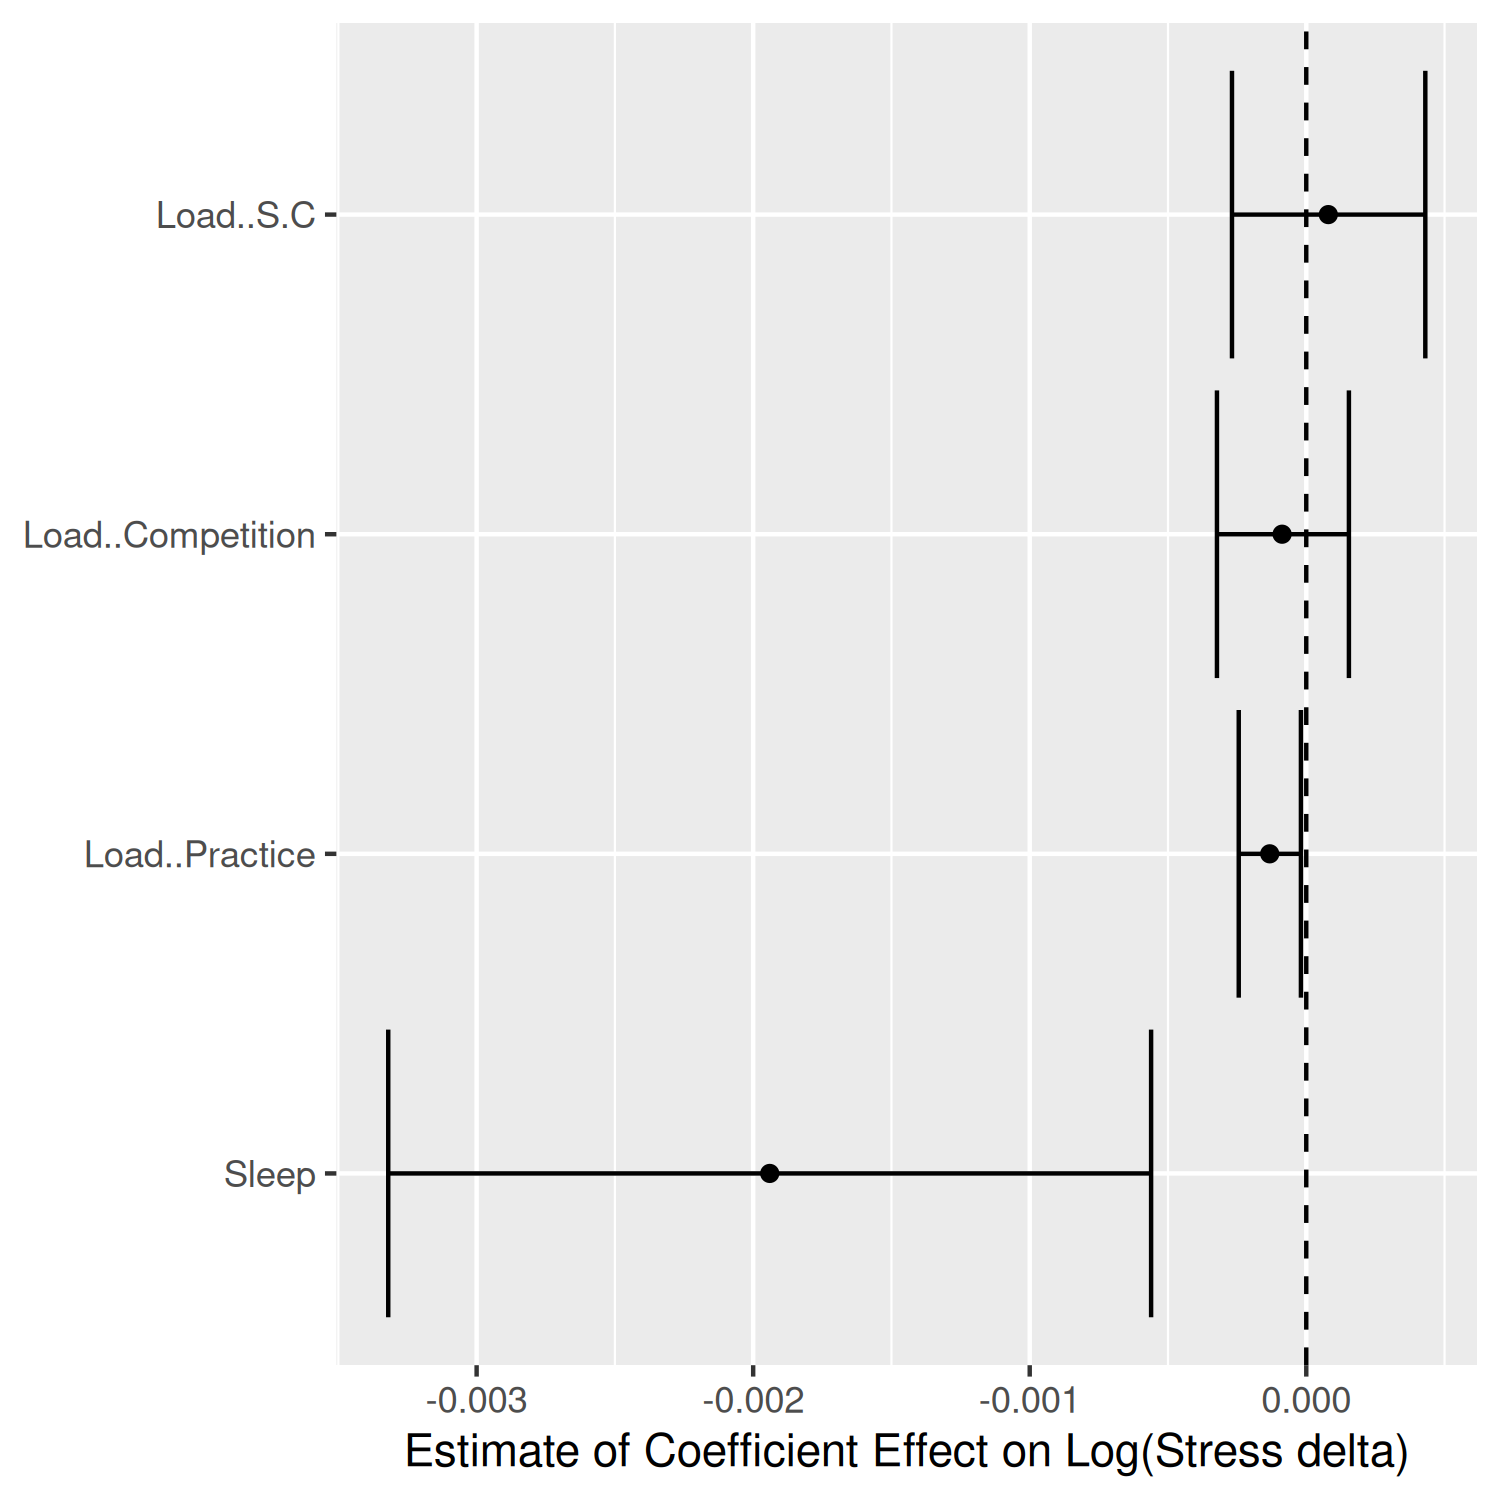
\includegraphics[
						width=12cm,
					]{../out/analysis_weekly_workload/workload_sleep_stress_delta/coef.png}
				\end{center}
				\caption{Coefficient magnitudes for gamma generalized linear regression
				of stress delta based on sleep and workload data.}
				\label{fig:weekly_workload_sleep_stress_delta_coef}
			\end{figure}

			\begin{figure}
				\begin{center}
					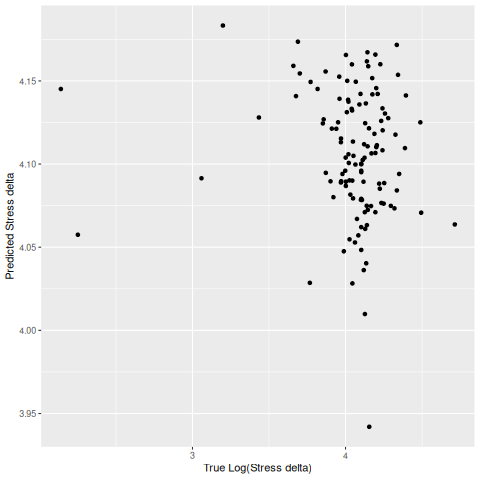
\includegraphics[
						width=12cm,
					]{../out/analysis_weekly_workload/workload_sleep_stress_delta/scatter_pred_true.png}
				\end{center}
				\caption{
					Scatterplot of predicted and true log-transformed outcome
					values for gamma generalized linear regression
					of stress delta based on sleep and workload data.
				}
				\label{fig:weekly_workload_sleep_stress_delta_scatter}
			\end{figure}

			% Fatigue.

			As shown in figure \ref{fig:weekly_workload_sleep_fatigue_coef}, sleep is
			by far the most impactful feature in terms of affecting an athlete's
			perceived fatigue level. Strength and conditioning workload may also
			be impactful, as neither of the two variables have a confidence interval
			overlapping with zero. Practice and competition loads have a much more
			modest effect. The accompanying model fit can be seen in
			figure \ref{fig:weekly_workload_sleep_fatigue_scatter}.

			% Fatigue delta.

			In terms of change in fatigue compared to the previous week, sleep
			is again the most impactful variable, being associated with decreased
			perceptions of fatigue from one week to the next. None of the other
			coefficients have confidence intervals that do not overlap with zero
			\ref{fig:weekly_workload_sleep_fatigue_delta_scatter}.

			% Mood.

			Mood is also positively affected by sleep, with the other three coefficients
			having comparatively very modest effects, if any at all
			\ref{fig:weekly_workload_sleep_mood_scatter}.

			% Mood delta.

			Concerning change in mood rating from week to week, sleep was the
			only variable whose coefficient confidence interval did
			not overlap with zero, suggesting a potential effect
			(see figure \ref{fig:weekly_workload_sleep_mood_delta_coef}).
			However, the associated model fit was poor (see figure
			\ref{fig:weekly_workload_sleep_mood_delta_scatter}).

			% Motivation.

			Sleep also positively affects motivation, being by far the most influential
			variable. The workload variables have a much lesser contribution, if any
			at all (see figure \ref{fig:weekly_workload_sleep_motivation_coef}).

			% Motivation delta.

			In the model fit for change in motivation from week to week, no
			coefficient had a confidence interval that did not overlap with zero
			(see figure
			\ref{fig:weekly_workload_sleep_motivation_delta_coef}). Additionally, the
			model fit was equivocal (see figure
			\ref{fig:weekly_workload_sleep_motivation_delta_scatter}).
			Hence, there does not appear to be an effect of any workload variable
			or sleep on the change in motivation from one week to another.

			% Stress.

			Stress appears to be negatively associated with sleep.
			Although no causal claims can
			be made on the basis of this analysis, and because stress often
			anecdotally co-occurrs with lower levels of sleep, it is difficult
			to determine whether one variable drives the other in the
			present context and athlete population. Interestingly,
			strength and conditioning load is also negatively associated with stress
			(see figure
			\ref{fig:weekly_workload_sleep_stress_coef}). However, the model fit here
			is somewhat poor, making it difficult to justify any firm conclusions on the
			basis of the data (figure \ref{fig:weekly_workload_sleep_stress_scatter}).

			% Stress delta.

			The model for change in stress from week to week had one of the least
			conclusive fits in the present analysis (see figure
			\ref{fig:weekly_workload_sleep_stress_scatter}). Therefore, firm
			conclusions cannot be made on the basis of the model fit.

		\subsection{Predicting Sleep Disturbance using Workload Data}

			\begin{figure}
				\begin{center}
					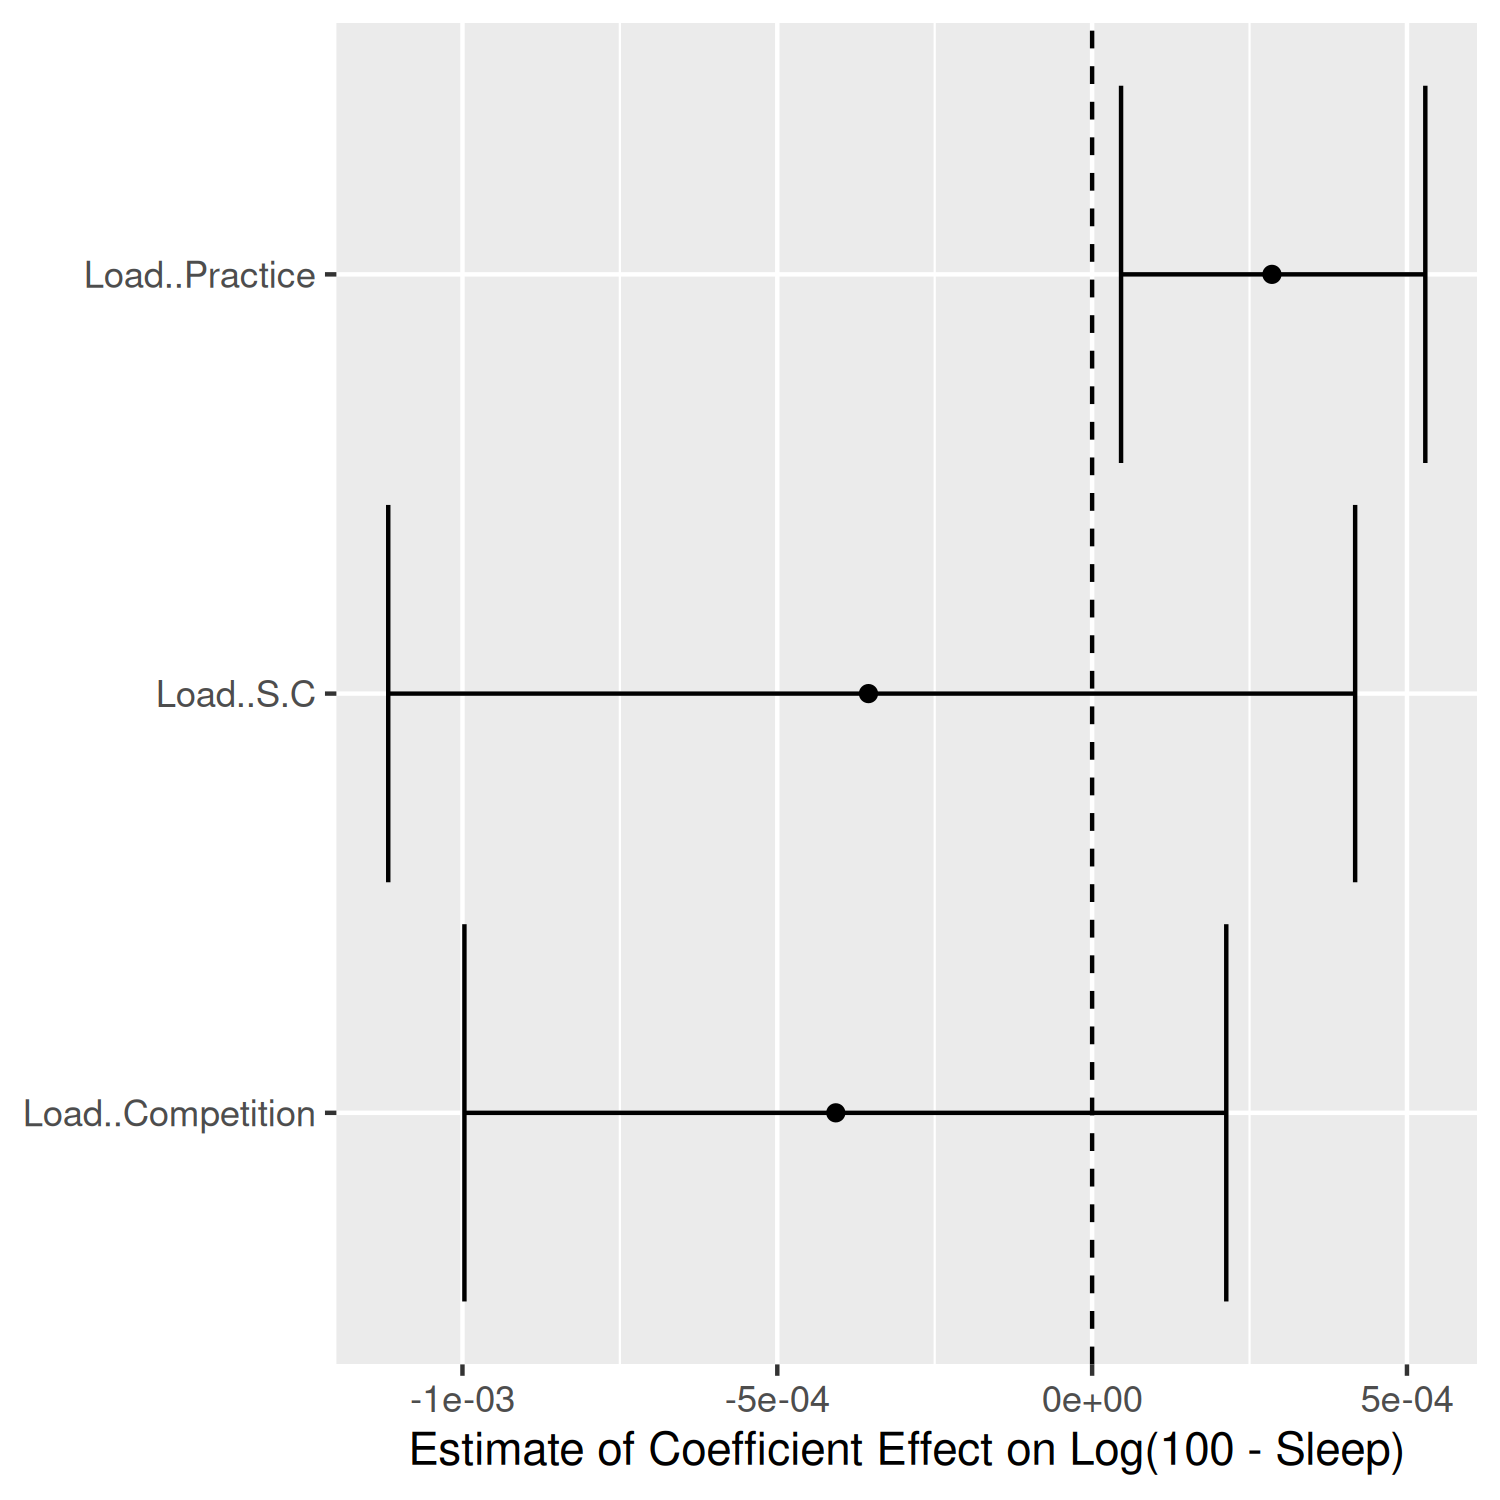
\includegraphics[
						width=12cm,
					]{../out/analysis_weekly_workload/workload_sleep/coef.png}
				\end{center}
				\caption{Coefficient magnitudes for gamma generalized linear regression
				of sleep based on workload data.}
				\label{fig:weekly_workload_sleep_coef}
			\end{figure}

			\begin{figure}
				\begin{center}
					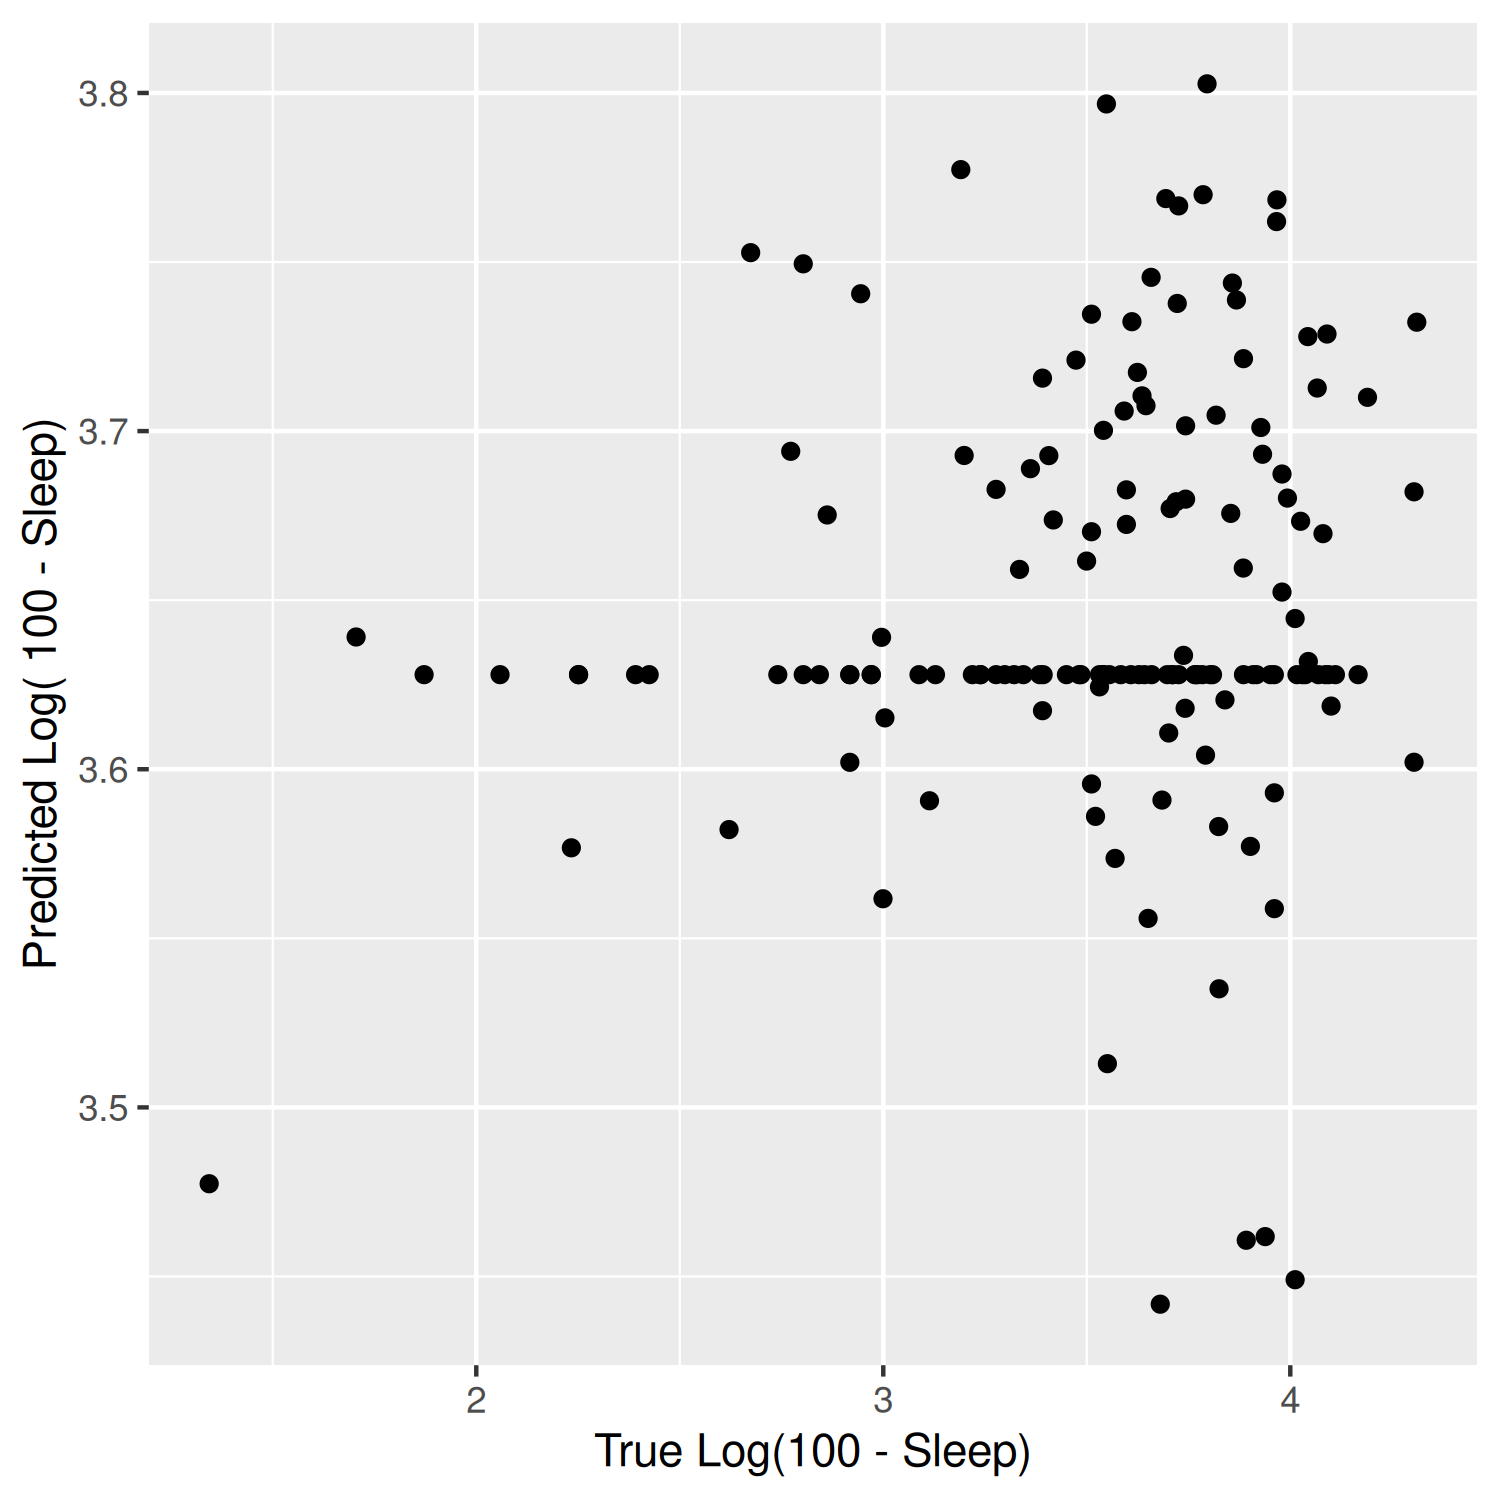
\includegraphics[
						width=12cm,
					]{../out/analysis_weekly_workload/workload_sleep/scatter_pred_true.png}
				\end{center}
				\caption{
					Scatterplot relating predicted sleep disturbance to
					true sleep disturbance.
				}
				\label{fig:weekly_workload_sleep_scatter}
			\end{figure}
			
			The quality of the model fit for sleep disturbance based on workload
			data is somewhat
			low due to the presence of many duplicate ground truth values.
			Tentatively, the null
			hypothesis can be retained that workload does not meaningfully affect sleep
			quality, with the possible exception of practice load.
			Although there may be physiological reasons to assume that this is
			not true, the data do not substantiate any strong relationship
			between workload and sleep disturbance in this cohort and time period.

		\subsection{Predicting Soreness using Workload, GPS, and Sleep}

			\begin{figure}
				\begin{center}
					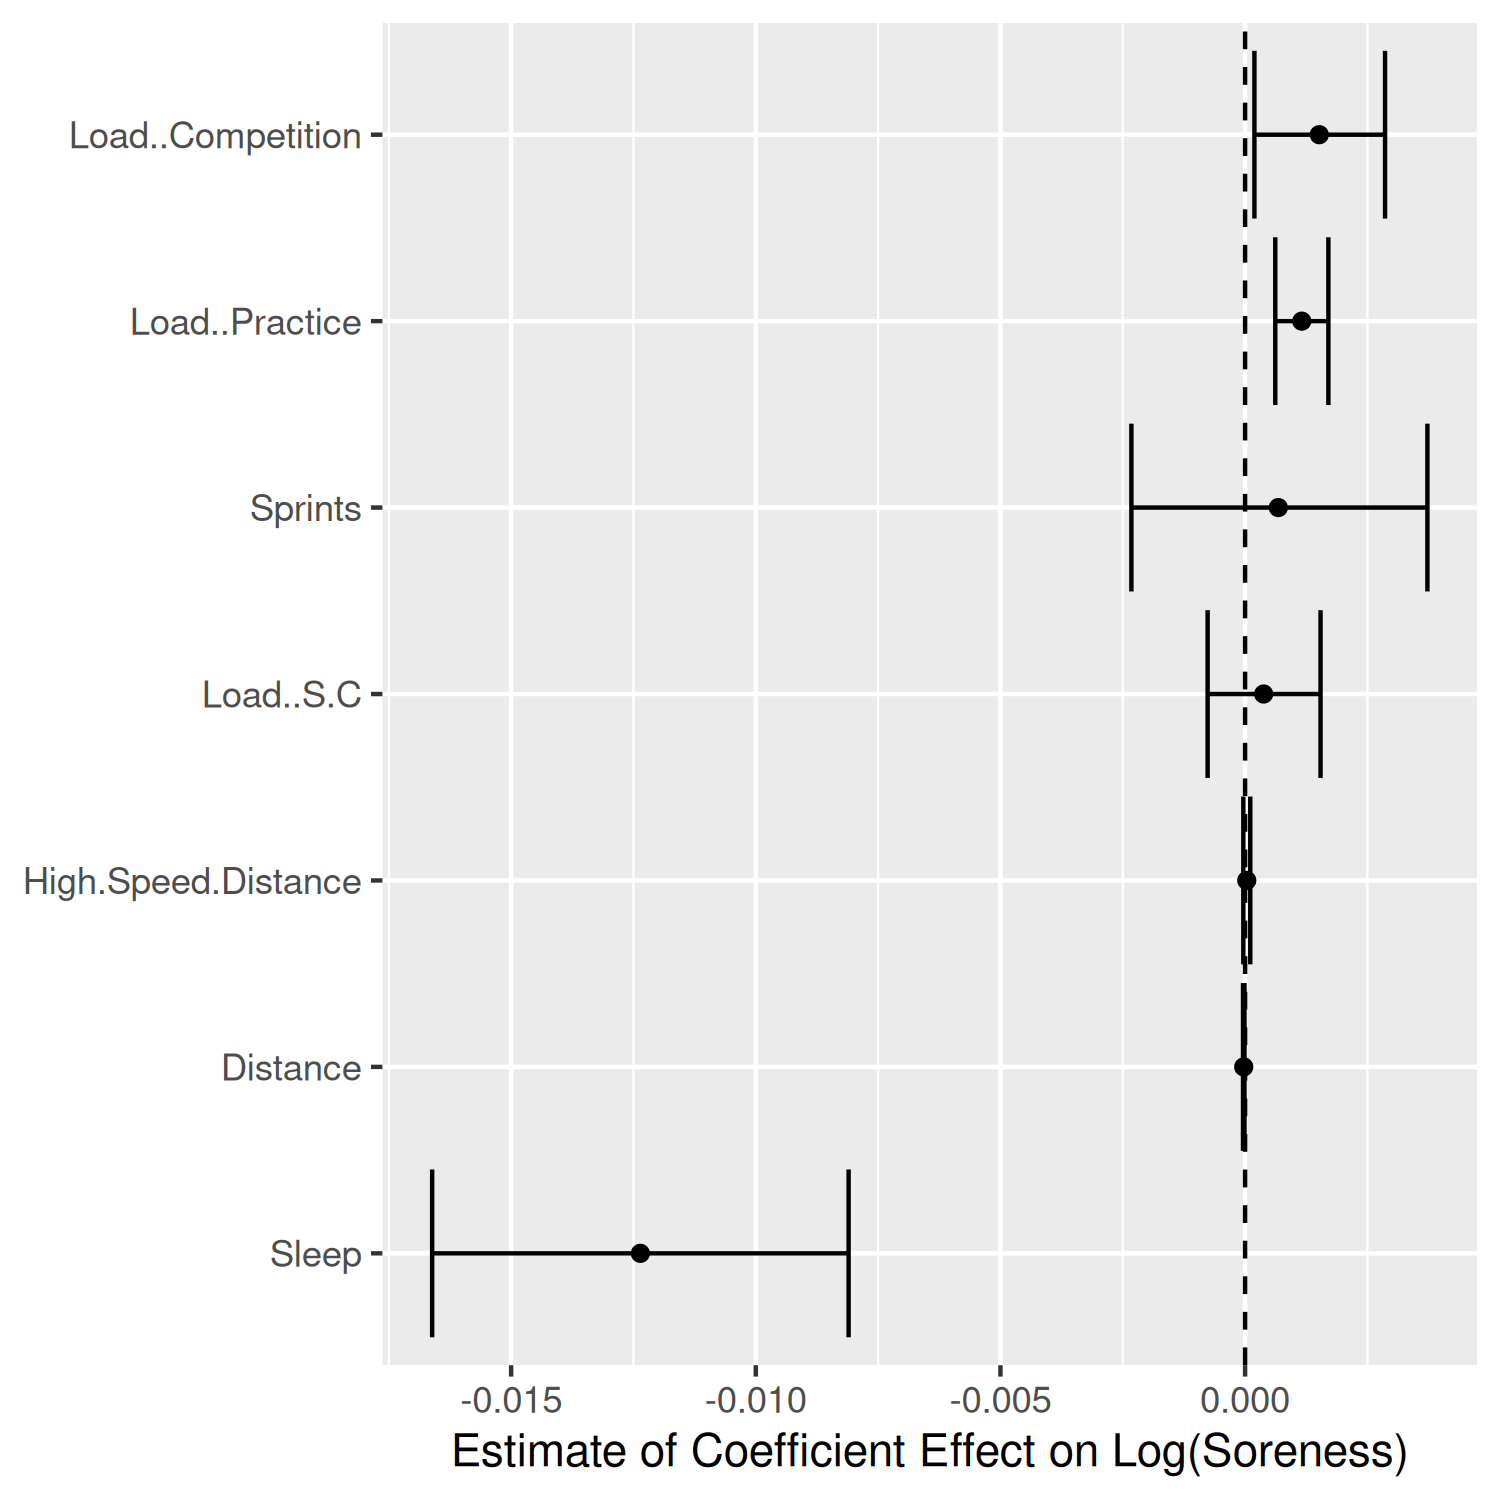
\includegraphics[
						width=12cm,
					]{../out/analysis_weekly_workload/workload_distance_sleep_soreness/coef.png}
				\end{center}
				\caption{Coefficient magnitudes for gamma generalized linear regression
				of sleep based on workload data.}
				\label{fig:weekly_workload_distance_sleep_soreness_coef}
			\end{figure}

			\begin{figure}
				\begin{center}
					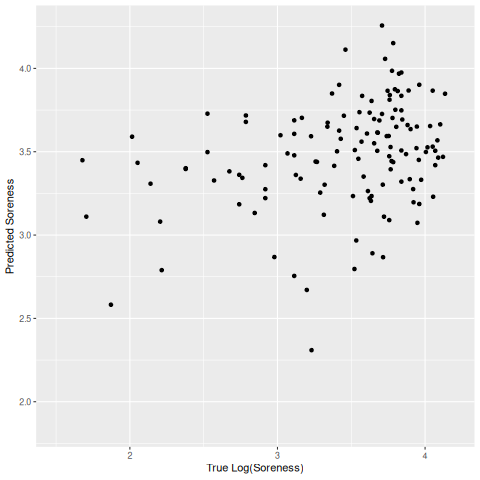
\includegraphics[
						width=12cm,
					]{../out/analysis_weekly_workload/workload_distance_sleep_soreness/scatter_pred_true.png}
				\end{center}
				\caption{
					Scatterplot relating predicted sleep disturbance to
					true sleep disturbance.
				}
				\label{fig:weekly_workload_distance_sleep_soreness_scatter}
			\end{figure}

			In predicting soreness on the basis of sleep, load, and GPS data, sleep
			was once again the most powerful indicator of how sore athletes would be
			in a given week. Competition load may also be positively associated
			with soreness, having a confidence interval that did not overlap with zero
			(see figure \ref{fig:weekly_workload_distance_sleep_soreness_coef}).

	% \section{Discussion}

	% 	Overall, sleep is the most potent influence over athlete wellbeing. Although
	% 	other variables do occassionally demonstrate potential effects, (e.g.,
	% 	competition load potentially positively affecting soreness, see)

	\section{Conclusion}
	
		\subsection{Key Insights and Action Items}

			\begin{itemize}
				\item EDA demonstrated that average session heart rate and
				practice load likely express much of the same information.
				If collecting both is logistically intractable or difficult,
				not much is lost by sacrificing one. Because of the familiarity
				of heart rate data and zones, it may be more useful to present
				these values to coaches and athletes.
				\item Sleep has by far the most outsized effect in promoting
				athlete wellness by reducing fatigue and stress and increasing
				mood and motivation (see figures
				\ref{fig:weekly_workload_sleep_fatigue_coef} through
				\ref{fig:weekly_workload_sleep_stress_delta_scatter}).
				\item Workload does not appear to affect sleep quality within
				the ranges in which it has been administered (figure
				\ref{fig:weekly_workload_sleep_coef}), with the exception of a potential
				slight effect for practice load.
				\item Soreness was negatively associated with sleep to a much
				greater degree than with any other variable (see
				\ref{fig:weekly_workload_distance_sleep_soreness_coef}).
				Competition load may positively influence soreness.
				\item There was an association between greater
				strength and conditioning load and lower levels of fatigue
				and stress (figures \ref{fig:weekly_workload_sleep_fatigue_coef},
				\ref{weekly_workload_sleep_stress_coef}).
				However, this effect is likely very slight and possibly
				confounded by position-based factors; for example, it may be
				the case that positions that engage in more strength and
				conditioning perform less other training.
				\item To promote athlete well-being, facilitating proper
				restful sleep should be considered one of the highest priorities,
				especially during circumstances of travel and international
				competition. Very
				secondarily, the inclusion of resistance training may help to
				reduce levels of fatigue and stress. Finally, since soreness is
				associated with high competition load, techniques to mitigate
				this trend may be beneficial for performance. For example,
				during periods of dense competition frequency when acute
				performance is prioritized over chronic adaptation, utilizing
				recovery modalities that reduce soreness may enhance performance.
			\end{itemize}

		\subsection{Directions for Future Work}

			One question which this report has not addressed is the extent
			to which the variation in the given workload and wellness data is simply a
			function of athlete position group. Although there are some trends
			which apply across the athlete groups (e.g., the impact of sleep),
			and while there are certainly athletes within a particular group
			that might not be best served by a model of their
			workload and wellness that relies on their position group alone, there
			are probably some trends that could provide helpful coaching heuristics.
			This could be a fruitful direction for further investigation.

			Very relatedly, it would be interesting to see if there are
			underlying latent positions that are different from those presented
			here. Principal component analysis or stochastic neighbor
			embedding (see \cite{hinton2002stochastic}) could help discover if there
			are more underlying positions than those described by the position
			groups.
			Otremba \cite{otremba2022smartpitch} did something very similar
			with pitch categories in SmartPitch. Using manifold learning techniques
			as outlined there could provide some direction to create more tailored
			recommendations based on such underlying groups.

			Additionally, the palette of models applied to the present task could
			be expanded, potentially resulted in improved outcomes.
			The generalized linear model with the gamma family of outcome
			variable distribution was chosen because
			of the observed density of the outcome variables included in
			the given data. This is valuable
			from an inferential standpoint, as models with assumptions that are
			most appropriate to the data are most suited for inferential
			claims about the individual coefficients. However, it may be that
			a Bayesian ridge regression, random forest regressor, or even
			basic multilayer perceptron would outperform the generalized linear
			model in terms of prediction accuracy. Whether or not the tradeoff
			in interpretability is worthwhile for these models would depend
			somewhat on the magnitude of the increase in prediction accuracy.
			However, this tradeoff could also be ameliorated to some degree
			with the use of Shapley values \cite{vstrumbelj2014explaining}.
			Additionally, it is questionable whether the outcomes are really
			gamma-distributed at all, especially given that they are expressed
			on a scale from 0-100. Strictly speaking, sampling from a gamma
			distributed variable cannot produce values equivalent to 0 and
			should not have a hard arbitrary upper limit the way that these
			outcome variables do. Hence, expanding the assumptions surrounding
			the distribution of the outcome variable could produce better
			fits and unlock further insights.

	\bibliography{report_sports_science.bib}
	\bibliographystyle{unsrt}

\end{document}

